
% \newcommand{\DraftOrFinal}{draft}
\newcommand{\DraftOrFinal}{final}

\documentclass[\DraftOrFinal,11pt,letter]{article}

\newcommand{\DSU}{{\sc Jvolve}}
\newcommand{\transformObject}{\texttt{jvolve\_object}}
\newcommand{\transformClass}{\texttt{jvolve\_class}}
\newcommand{\VMClass}{\texttt{VM\_Class}}
\newcommand{\TIB}{\texttt{TIB}}
\newcommand{\JTOC}{\texttt{JTOC}}
\newcommand{\GroupC}{\suriya{Some name for Group C}}
\newcommand{\JikesRVM}{Jikes RVM}

\usepackage{acronym}
\usepackage{multirow}
\usepackage{epsfig}
\usepackage{fullpage}
\usepackage{float}
\usepackage{setspace}
\usepackage{url}
\usepackage{srcltx}
\usepackage[\DraftOrFinal,inline]{showlabels}
\usepackage{hyperref}
\usepackage{ifdraft}
\usepackage[usenames]{color}
\usepackage[override]{cmtt}
% \usepackage[centering,scale=0.80]{geometry}
% \usepackage{nopageno}
% \usepackage{array}

\ifdraft{
\newcommand\maybecolor[1]{\color{#1}}
\newcommand\mwh[1]{[{\maybecolor{red}\textbf{Mike says:} #1}]}
\newcommand\ksm[1]{[{\maybecolor{red}\textbf{Kathryn says:} #1}]}
\newcommand\suriya[1]{[{\maybecolor{blue}\textbf{Suriya says:} #1}]}
}{
\newcommand\mwh[1]{}
\newcommand\ksm[1]{}
\newcommand\suriya[1]{}
}

\begin{document}

\title{
       Dynamic Software Updates for Java:\\ A VM-Centric Approach\\
       \vspace{+0.5em}
       Ph.D. Proposal}

\author{Suriya Subramanian \\
        Department of Computer Sciences \\
        The University of Texas at Austin}

\date{July 21, 2008}

\maketitle

\subsection*{Abstract}
Software evolves to fix bugs and add features. Stopping and restarting
programs to apply changes is inconvenient and often costly.  Dynamic
software updating (DSU) addresses this problem by updating programs
while they execute, but existing DSU systems for managed languages do
not support many updates that occur in practice and are inefficient.
This paper presents the design and implementation of \DSU, a
DSU-enhanced Java VM.  Updated programs may add, delete, and replace fields
and methods anywhere within the class hierarchy.  \DSU{} implements
these updates by adding to and coordinating VM classloading,
just-in-time compilation, scheduling, return barriers, on-stack
replacement, and garbage collection.  \DSU{} is \emph{safe}: its use
of bytecode verification and VM thread synchronization ensures that an
% ISSUE: no bytecode verification in JikesRVM
update will always produce type-correct executions. \DSU{} is
\emph{flexible}: it can support 20 of 22 updates to three
open-source programs---Jetty web server, JavaEmailServer, and CrossFTP
server---based on actual releases occurring over 1 to 2 years.
%REFACTOR: though slight refactorings would allow the other updates.
\DSU{} is \emph{efficient}: performance experiments show that
\DSU{} incurs \emph{no overhead} during steady-state execution.  These
results demonstrate that this work is a significant step towards
practical support for 
dynamic updates in virtual machines for managed languages.

%%% Local Variables: 
%%% mode: latex
%%% TeX-master: "pldi64"
%%% End: 


% {
% \setbeamertemplate{headline}{}
% \setbeamertemplate{footline}{}
% \setbeamertemplate{navigation symbols}{}
% \begin{frame}
% \begin{block}{}
% \begin{quote}
% The only thing that is constant is change.\\
% \hfill Heraclitus of Ephesus
% \end{quote}
% \end{block}
% \end{frame}
% }

% \section{Introduction}
% \subsection{Motivation}
\begin{frame}{Motivation}%{A Sub-title is optional}
\begin{itemize}
\item Software applications change all the time
\item Deployed systems must be updated with bug fixes, new features
\item Updating typically involves: stop, apply patch, restart
% \vspace{1ex}
% \begin{center}\begin{Huge}Updating $\Rightarrow$ Downtime\end{Huge}\end{center}
\item Not desirable
  \begin{itemize}
    \item Safety concerns
    \item Revenue loss
    \item Inconvenience
  \end{itemize}
\end{itemize}
% \item Might not be affordable for some applications
%   \begin{itemize}
%   \item Applications that retain state that cannot be externalized
%   \end{itemize}
\end{frame}

\begin{frame}{Dynamic software updating}%{A Sub-title is optional}
\vspace*{-3mm}%
\begin{center}%
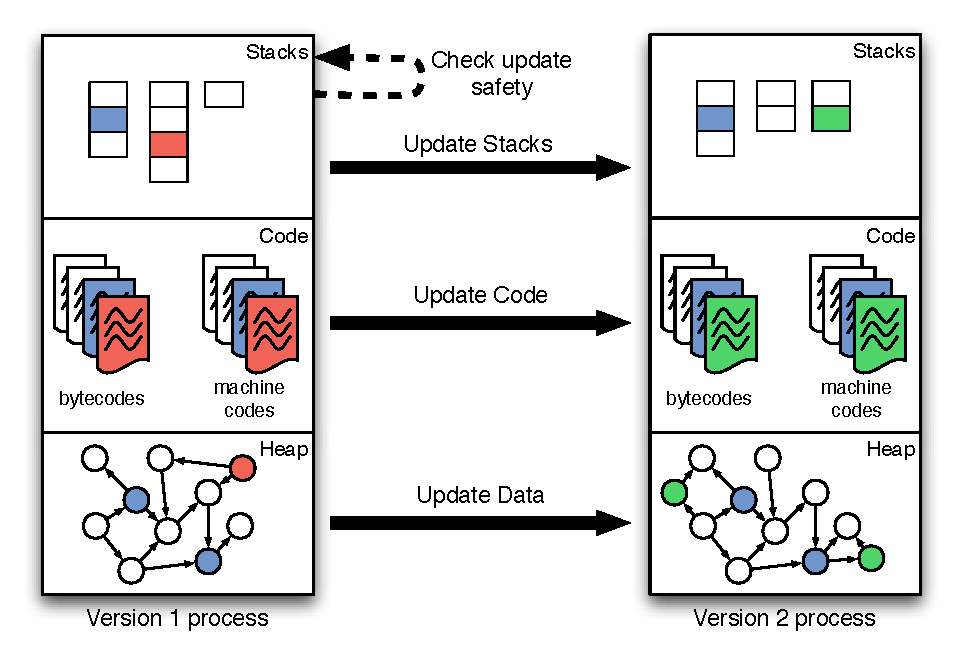
\includegraphics[scale=0.73]{images/process-state/both-process-state}%
\end{center}%
\end{frame}

\begin{frame}{Dynamic updating systems}%{A Sub-title is optional}
\begin{itemize}
\item Special-purpose architectures, application-specific solutions exist
\item General-purpose solutions gaining strength
  \begin{itemize}
  \item K42, Ksplice for OS updates
  \item Polus, Ginseng for C applications
  \end{itemize}
\item Not for managed languages
\end{itemize}
\end{frame}

% \begin{frame}{Motivation}%{A Sub-title is optional}
% \begin{itemize}
% \item Software applications change all the time
% \item Deployed systems need to be updated
% \item Some systems cannot afford downtime (safety concerns, revene loss),
% many systems perfer to avoid downtime (inconvenience)
% \item Stopping, updating and restarting deployed systems is not ideal
% \item Neither is delaying critical updates
% \end{itemize}
% \end{frame}

% \begin{frame}{Motivation}%{A Sub-title is optional}
% \begin{itemize}
% \item 75\% of downtime in high-availablity applications is for planned
% maintenance
% \uncover<2->{
% \item Personal operating system
% \item Enterprise applications
% \item Telecommunication, transportation systems
% % \uncover<3->{
% % \item Even a cache with lots of state
% %   \begin{itemize}
% %   \item LinkedIn.com architecture\footnote{\scriptsize{\url{http://hurvitz.org/blog/2008/06/linkedin-architecture}}}
% %   \item ``The Cloud'': In memory representation of the LinkedIn network graph
% %   \item Network size - 22M nodes, 120M edges
% %   \item Rebuilding an instance takes 8 hours
% %   \end{itemize}
% % }
% }
% \end{itemize}
% \end{frame}

% % \subsection{Solutions}
% \begin{frame}{Conventional solutions to avoid downtime}%{A Sub-title is optional}
% \begin{itemize}
% \item Move state out of the process, for instance databases
% \item Use multiple processes, and do a rolling update
% \end{itemize}
% \uncover<2>{
% \begin{itemize}
% \item Not always possible
% \item Restricted to specific application domains
% % \item DSU is a generic solution
% \end{itemize}
% }

% \begin{frame}{Dynamic Software Updating}%{A Sub-title is optional}
% Updating state of a process on the fly
% \begin{itemize}
% \item Special purpose techniques/architectures work, but we want a general
% solution
% \item 
% \end{itemize}
% \end{frame}

%   \begin{itemize}
%   \item State stored externally, for instance databases
%   \item Redundant systems: start a new process and stop this one
%   \item Not always possible
%   \end{itemize}
% \item<2-> Dynamic Software Updating (DSU)
%   \begin{itemize}
%     \item Update process state without restarting application
%     \item Non-redundant systems benefit as well
%     \item Decouples fault-tolerance from software updating
%   \end{itemize}
% \end{frame}

% \begin{frame}{Process state}%{A Sub-title is optional}
% \vspace*{-2ex}\includegraphics[scale=0.72]{images/process-state}
% \end{frame}

% \begin{frame}{DSU requirements}%{A Sub-title is optional}
% % \begin{center}
% % A Dynamic Software Updating solution should \emph{ideally} be
% % {\bf safe}, {\bf flexible}, and {\bf efficient}.
% % \end{center}
% \begin{description}
% \item[Safe] Updating is as correct as starting from scratch
% \item[Flexible] Support changes encountered in practice
% \item[Efficient] No performance impact
% \end{description}
% \end{frame}

% \begin{frame}{State of the art}%{A Sub-title is optional}
% Significant progress for C
% \begin{itemize}
% \item Server feature upgrades
%   \begin{itemize}
%   \item Ginseng \cite{neamtiu06dsu}
%   \item POLUS \cite{chen:icse07}
%   \end{itemize}
% \item Security patches: OPUS \cite{altekar05opus}
% \item Operating system upgrades
%   \begin{itemize}
%   \item K42 \cite{K42reconfig}
%   \item DynAMOS \cite{dynamos_eurosys_07}
%   \item LUCOS \cite{chen06vee}
%   \item Ksplice \cite{Ksplice}
%   \end{itemize}
% \end{itemize}
% % \item<2-> Primitive support for managed languages
% %   \begin{itemize}
% %   \item Very restrictive
% %   \item Space and time overheads
% %   \item Not proven on realistic applications
% %   \end{itemize}
% \end{frame}

% \begin{frame}{DSU opportunity for managed languages}%{A Sub-title is optional}
% DSU Solutions for C/C++ typically
% \begin{itemize}
% \item Require special compilation
% \item Statically/dynamically insert indirection for function calls
% \item Restrict structure updates, require extra allocation
% \item Impose space/time overheads on normal execution
% \item Make type-safety for updates difficult
% \item Not multi-threaded
% \end{itemize}
% \end{frame}

% \begin{frame}{Possible DSU solutions}%{A Sub-title is optional}
% Achieve DSU support by
% \begin{itemize}
% \item Making the application DSU-aware
% \item Special recompilation
% \item A class loader based colution 
% \item DSU support in the VM
% \end{itemize}
% \end{frame}

% \begin{frame}{Related work}%{A Sub-title is optional}
% \begin{itemize}
% \item Custom class loader solutions:\\Eisenbach and Barr, Milazzo et al.
% \item Source-to-source translation: Orso et al.
% \item VM-based solutions: JDrums, Dynamic Virtual Machine (DVM)
% \item In a persistent object store: Boyapati et al.
% \end{itemize}
% \uncover<2>{
% \begin{itemize}
% \item Limited, not flexible
% \item Restricted data-transformation model (like requiring {\em encapsulation} based
% on {\em ownership types})
% \item Overhead during normal execution
% \end{itemize}
% }
% \end{frame}

% \begin{frame}{Existing solutions for managed languages}%{A Sub-title is optional}
% \begin{itemize}
% \item VM-based solutions
%   \begin{itemize}
%   \item JDrums \cite{ritzau00dynamic}, DVM \cite{Mala00a}
%   \item Not well evaluated
%   \item Provide an interface similar to \DSU{}
%   \item Perform lazy updates
%   \item Overheads during normal execution
%   \end{itemize}
% \item Standard VM with DSU support
%   \begin{itemize}
%   \item DJVCS \cite{BarrE03}, DUSC \cite{orso:java}, \cite{Milazzo05updates}
%   \item Special classloaders, compilers
%   \item Very restrictive
%   \item Space/time overheads
%   \end{itemize}
% \end{itemize}
% 
% \end{frame}

% \begin{frame}{Related work}%{A Sub-title is optional}
% Nobody can beat us.
% \end{frame}

\begin{frame}{Our solution}%{A Sub-title is optional}
\begin{itemize}
\item \DSU{} - a Java Virtual Machine with DSU support
% \item Built on top of Jikes RVM, a Java-in-Java VM
\item Key insight: Extend existing VM services
%   \begin{itemize}
%   \item Classloading
%   \item Bytecode verification%\footnote{Jikes RVM does not have a bytecode verifier}
%   \item Thread synchronization
%   \item JIT Compilation
%   \item On-stack replacement
%   \item Garbage collection
%   \end{itemize}
\item No DSU-related overhead during normal execution
\item Support updates to real world applications
\begin{block}{}
\emph{Dynamic software updating in managed languages can be achieved in a
{\bf safe}, {\bf flexible} and {\bf efficient} manner by naturally extending existing VM
services.}
\end{block}

\begin{block}{}
\emph{DSU support should be a standard feature of future VMs.}
\end{block}
\end{itemize}
\end{frame}

% \begin{frame}{Contribution}%{A Sub-title is optional}
% \setbeamercovered{invisible}
% \begin{block}{}
% \emph{Dynamic software updating in managed languages can be achieved in a
% {\bf safe}, {\bf flexible} and {\bf efficient} manner by naturally extending existing VM
% services.}
% \end{block}
% 
% \begin{block}<2->{Corollary}
% \emph{DSU support should be a standard feature of future VMs.}
% \end{block}
% \end{frame}

\section{Related Work}

We discuss related work on supporting DSU in managed
languages and in C and C++. DSU for managed
languages falls into two categories: special-purpose VMs and libraries
and/or classloader-inserted or compiler-inserted code modifications.
Support for DSU in C and C++ often combines compiler and runtime
system support.  Existing approaches widely vary in their update
flexibility, safety guarantees, and run-time overhead.

% Broadly speaking, \DSU{} is one of the most flexible systems proposed
% to date, and % when compared to systems with similar flexibility,
% demonstrates superior performance and a realistic and thorough
% evaluation. 

\paragraph{Edit and Continue Development}

Debuggers have long provided \emph{edit and continue} (EnC)
functionality that permits
limited modifications to program state to avoid stopping and
restarting during debugging. For example, Sun's HotSwap
VM~\cite{JVMhotswap,Dmit01a}, .NET Visual Studio for C\# and
C++~\cite{VSEnC}, and library-based support~\cite{eaddy05enc} for .NET
applications all provide EnC.  These systems are all less flexible than
\DSU, typically supporting only code changes within method bodies.
This limitation reduces safety concerns, and programmers need not write
class or object transformers, but as discussed in
Section~\ref{sec:experience}, more than half of the updates we saw in
practice would be disallowed. 

%% As a vehicle for ``fix \& continue'' this is really popular!  Just Google
%% for edit and continue .net.  There was a big uproar when the feature was
%% taken away.

% \paragraph{DSU in Managed Languages}

%Approaches that implement DSU for managed languages can be divided into two
%categories: those that employ a special-purpose VM, and those based on
%compiler and/or library support.

% \paragraph*{Approaches with special VM support.}

\paragraph{Special VM support for DSU}

JDrums~\cite{ritzau00dynamic} and Dynamic Virtual Machine
(DVM)~\cite{Mala00a} both implement DSU support for Java within the
VM, providing a programming
interface similar to \DSU.  However, their implementations impose
overheads during normal execution, whereas \DSU{} has zero overhead
and a richer evaluation.
Both prior VMs update \emph{lazily}.  For example, JDrums traps object
pointer dereferences to check whether a new version of the object's
class is available. If so, the VM runs the object transformer
function(s) to upgrade the object.  By contrast \DSU{} performs
updates eagerly, as part of a full heap GC\@. DVM performs updates
lazily as JDrums, but does some eager conversion incrementally.  Lazy
updating has the advantage that the pause due to an update can be
amortized over subsequent execution.

The main drawback is that the overhead persists during normal execution
even though updates are relatively rare. \ksm{TODO: say why so much.}

Both JDrums and DVM are in the Sun JDK 1.2 VM, which uses an extra
level of indirection (the \emph{handle space}) to support heap
compaction.  Indirection conveniently supports object updates, but
adds additional space and time overhead.  DVM only works with the interpreter.
Relative to the stock bytecode interpreter, which is already slow, the
extra traps result in roughly 10\% overhead.  By contrast, \DSU{}
imposes no overhead before or after an update.  Neither JDrums nor
DVM has been evaluated on updates derived from realistic
applications. % ---only a handful of toy updates have been considered.
% Papers on 
% JDrums present only a toy phone book example and the DVM paper reports
% no experience at all.

%\suriya{is this a bit too strong?} \ksm{nope}

%% JDRUMS: implements the conversion lazily.  They have a similar interface
%% (object and class transformers). The drawback here is that there is overhead
%% in the general case of execution---we do not know when the update is
%% complete.  Implemented in Sun's JDK 1.2.  Adds a level of indirection to the
%% new object.  Thus overhead builds up over time.  It also appears they have a
%% more limited interface to what can be referenced in a conversion function.
%% For example, there is no way to refer to fields other than those of the
%% object's class (i.e., no super-class fields) and there is no way to call new
%% methods, like constructors.  Not clear if there are restrictions on how
%% methods can be changed.

%% DVM: use an incremental mark-sweep collector, where mark phase marks objects
%% to be updated and the sweep phase incrementally updates them (prior to being
%% accessed by the mutator).  Like JDRUMS, all accesses to marked objects are
%% trapped.  Imposes a stock 10\% overhead, even only using bytecode.

%% Both of these: no significant experience with real applications, according
%% to how they change in practice.  They also can't handle native methods
%% because they can't trap access to modified objects.  Doing the full GC
%% solves this problem.

% More recently, Nicoara et al. developed PROSE, a system for run-time
PROSE performs run-time
code patching with an API in the style of aspect-oriented
programming~\cite{nicoara:eurosys08}.  PROSE aims to support
short-term, run-time patches to code for logging, introspection, or
performance adaptation, rather than for DSU. % in support of run-time software
As such, PROSE only supports updates to method bodies,
with no support for signature or state changes. % This flexibility is
% similar to the EnC implementations discussed above; 
% indeed, PROSE builds on the HotSwap method replacement support in its
% Sun JDK implementation~\cite{JVMhotswap}.

Gilmore et al.~\cite{GilmoreKW97} propose DSU support for modules in
ML programs. They use a programming interface that is similar to ours, but
more restrictive.  They also propose using copying GC to perform the
update, as we do.  They formalized an abstract machine for
implementing updates using a copying garbage collector, but did not
implement it.

 
Boyapati et al.~\cite{boyapati03lazy} support lazily upgrading objects
in a \emph{persistent object store} (POS).  Though in a different
domain, their programming interface is quite similar to \DSU{} and the
other Java-based systems: programmers provide object transformer
functions for each class whose signature has changed.  In their system, object
transformers % are somewhat different than ours.  Their system
% allows the object transformer of some class $A$ to access the state of
of some class $A$ may access the state of
old objects pointed to by $A$'s fields, assuming these objects are
fully encapsulated; i.e., they are only reachable through $A$.
Encapsulation is ensured via extensions to the type system.  By
contrast, our transformers may dereference fields via old objects, but
if these fields point to objects whose classes have been updated, they
will see the \emph{new} versions. % (a semantics which is more
% typical).
We plan to explore the costs/benefit trade-off of these
semantics in future work.
%% To avoid programmer annotations we could use a tool like Uno


% \paragraph*{Approaches using a standard VM.}
\paragraph{Standard VM, with support for DSU}
To avoid changing the VM, researchers have developed special-purpose
classloaders, compiler support, or both for DSU.  The main drawbacks
of these approaches are less flexibility and greater
overhead.  Eisenbach and Barr~\cite{BarrE03} and Milazzo et
al.~\cite{Milazzo05updates} use custom classloaders to allow
binary-compatible changes and component-level changes, respectively.
The former targets libraries and the latter is part of the design of a
special-purpose software architecture.

%% Eisenbach and Barr: safe upgrading without restarting.  They support
%% upgrades that satisfy binary compatibility.  Uses a custom classloader and
%% JMX to replace the code of existing objects.  No way to modify the state of
%% the objects.

%% Milazzo use a modified class loader to load individual replacements to
%% classes in a special-purpose architecture.  The class loader may modify the
%% bytecode of the loaded class to deal with type version namespace issues.
%% Basically this is more limited in scope than our approach.

Orso et al.~\cite{orso:java} support DSU via source-to-source translation
by introducing a proxy class that indirects accesses
to objects that could change.  
%% For each class C that might change in the future they produce a proxy for
%% that class.  All calls from clients of C are redirected to call the wrapper
%% instead.  When C is updated by some new class C', a new C' object is created
%% and initialized using the old state of C and the wrapper is redirected to
%% point to C'.
This approach requires updated classes to export the same public
interface---it forbids new non-private methods and fields. % can be added to an
A more general limitation of non VM-based approaches
is that they are not \emph{transparent}---they make changes to the
class hierarchy, insert or rename classes, etc.  This approach makes
it essentially impossible to be robust in the face of code using
reflection or native methods.  Moreover, the extra runtime support
imposes both time and space overheads.  By contrast, modifying the VM
is much simpler, given its existing services.  Our VM approach handles
native methods and reflection,
and is more expressive, e.g., supporting signature changes.

%% Run-time mod of class hierarchy in a live ...
%% -  Also a classloader-based approach.  Classloaders are used to manage the 
%% *** skip this

\paragraph{Dynamic Software Updating for C/C++}
\suriya{DSU or expansion in headings?}

Recently several substantial systems for dynamically updating C and
C++ programs have emerged that target server
applications~\cite{HjalmtyssonG98,altekar05opus,neamtiu06dsu,chen:icse07}
and operating systems
components~\cite{K42reconfig,k42usenix,chen06vee,lee06linuxmod,dynamos_eurosys_07}.
% These systems are more mature than most of the systems described above, in
% some cases with substantial updating experience.  The flexibility

Although these systems are mature, the flexibility
afforded by \DSU{} is comparable or superior to most of them.
Only Ginseng~\cite{neamtiu06dsu} imposes fewer restrictions
on update timing than \DSU, but all these systems
cannot update multi-threaded programs or handle object-oriented language
features.

The lack of a VM is a significant disadvantage % in the implementation
for C and C++ DSU.  For example, because a VM-based \acs{JIT} can compile
and recompile replacement classes, it can update them with no
persistent overhead.  By contrast, C and C++ implementations must use
either statically-inserted
indirections~\cite{HjalmtyssonG98,neamtiu06dsu,K42reconfig,k42usenix}
or dynamically-inserted trampolines to redirect function
calls~\cite{altekar05opus,chen06vee,chen:icse07,Ksplice}.  Both cases impose
persistent overhead on normal execution, % in and of themselves, and can
and inhibit optimization.  Likewise, because these systems lack a garbage
collector, they either do not update object instances at
all~\cite{Ksplice}, update them
lazily~\cite{neamtiu06dsu,chen:icse07} or perform extra allocation and
allocator bookkeeping to be able to locate the objects at
update-time~\cite{k42usenix}.  Both of the latter two approaches impose time and space
overheads on normal execution, whereas \DSU{}'s VM-based approach has
no a priori overheads.  Finally, the fact that C and C++ are not
type-safe greatly complicates efforts to ensure that updates behave
correctly.

%% basic swapping for single modules.





\begin{figure}[t]
\begin{center}
\scalebox{.67}{\includegraphics{images/system}}
\end{center}
\caption{Dynamic Software Updating with \DSU}
\label{fig:overview}
\end{figure}


%MWH: I don't think this section is particularly about a VM-centric
%   design.  I've reverted the text back to the way it was.  The next
%   section is about the VM.  We'd have to make more significant
%   changes here, not sure how, to somehow claim this is an overview
%   of VM-centric DSU.  The approach here, modulo the discussion of
%   garbage collection, could just as well apply to a system
%   implemented via rewriting.

% \section{A VM-centric DSU Design}

% This section begins by overviewing a VM-centric approach, our design
% choices, update model, and describes how the developer participates in
% the process. Section~\ref{sec:vm} describes each component in detail.

\section{Dynamic Updates in \DSU}

This section overviews \DSU's approach, what changes it permits, and
how the developer participates in the process.

\subsection{System Overview}
\label{sec:overview}

Figure~\ref{fig:overview} illustrates the dynamic update process.
Assume that the VM is executing the current version of the program,
whose code is depicted in the left top corner.  Meanwhile, developers
prepare a new version and fully test it using standard procedures.
A developer 
then invokes \DSU's \ac{UPT} on the old and
new versions. The \ac{UPT} generates an update specification, which identifies
new and updated classes, and a \texttt{JvolveTransformers.java} file
that contains default \emph{object}
and \emph{class transformer} methods.  

Transformer methods take an
object or class of the old version and 
initialize the corresponding object or class of the new version.  The default
transformers assign default values, such as zero and {\tt null}, to new
instance, reference, and static fields, and copy values for unchanged
fields.  Developers may customize the default transformers as
necessary.  We present an example update and transformer in
Section~\ref{subsec:transformers}. %, and briefly discuss how they are compiled.

The user signals the running VM to apply the update, and the VM loads
the new class files and transformers and schedules the update. The VM
scheduler signals an interrupt, which stops all threads at
VM safe points, where it is safe to perform thread scheduling and garbage collection.  \DSU{} then checks if the VM is % also
at a \emph{DSU safe point}. DSU safe points require that no thread's
activation stack contains a \emph{restricted} method.  Restricted
methods are of three categories: (1) methods changed by the update,
(2) methods whose bytecode is unchanged but whose compiled
representation may change, and (3) methods specified by the user. If
restricted methods are on stack, the VM installs return-barriers
for~(1) and~(3), and performs on-stack-replacement for~(2) to reach a
DSU safe point.  Section~\ref{sec:safe} describes this process in
detail.

Once all application threads have synchronized at DSU safe points, \DSU{}
applies the update. It first invalidates the compiled versions of all
changed methods.
These methods are
recompiled as needed---the adaptive JIT compiler will
generate code the next time the program invokes an invalidated method,
and may optimize it further, if the program executes it frequently.
%
The VM then invokes the
class transformers.  Finally, the VM initiates a full copying garbage collection. It
piggybacks on the garbage collector to detect all existing objects
whose classes change. It allocates objects that conform to the new type
declarations, and performs object transformations to populate the new
objects with valid state. %, as described above.  
At this point, the update is complete.

\begin{figure*}[t]
\begin{tabular}{c|c}
\begin{minipage}{3.12in}
\begin{small}
\begin{verbatim}
public class User {
  private final String username, domain, password;
  private String[] forwardAddresses;
  public User(...) {...}
  public String[] getForwardedAddresses() {...}
  public void setForwardedAddresses(String[] f) {...}
}
public class ConfigurationManager {
  private User loadUser(...) {
     ...
     User user = new User(...);
     String[] f = ...;
     user.setForwardedAddresses(f);
     return user;
  }
}
\end{verbatim}
\end{small}
\end{minipage} &
\begin{minipage}{3.5in}
\begin{small}
\begin{verbatim}
public class User {
  private final String username, domain, password;
  private EmailAddress[] forwardAddresses;
  public User(...) {...}
  public EmailAddress[] getForwardedAddresses() {...}
  public void setForwardedAddresses(EmailAddress[] f) {...}
}
public class ConfigurationManager {
  private User loadUser(...) {
     ...
     User user = new User(...);
     EmailAddress[] f = ...;
     user.setForwardedAddresses(f);
     return user;
  }
}
\end{verbatim}
\end{small}
\end{minipage} \\
(a) Version 1.3.1 &
(b) Version 1.3.2 \\
\end{tabular}
\caption{Example changes to JavaEmailServer \texttt{User} and
  \texttt{ConfigurationManager} classes}
\label{fig:email-example}
\end{figure*}

% vim:nospell


\subsection{Programmer Update Model}
\label{sec:updates}

We have designed a flexible, yet simple update model that supports
updates that we believe are important in practice. 

Programmers may
change method bodies. Method body updates are the simplest and most
commonly supported
change~\cite{JVMhotswap, VSEnC, eaddy05enc, GilmoreKW97, orso:java,
  K42reconfig, HjalmtyssonG98},
because DSU systems can preserve type safety by simply invoking the new
method the next time the program executes the method.  However,
restricting updates to method bodies prevents many common
changes~\cite{neamtiu05evolution}.  Section~\ref{sec:experience} shows
% Suriya: changed shows to will show
%MWH: this should be present tense.  A document always shows
%something.  It doesn't change, so what it shows in the future is the
%same as what it shows now.
that over half the releases of Jetty, JavaEmailServer, and CrossFTP
change more than just the method bodies.
%MWH: we haven't introduced what "class signature" means yet.

Programmers may also change class signatures in various ways.
They may change method signatures, e.g., by changing the type or
number of method arguments.  They may add or delete instance and
static field members and change the types or access modifiers of
existing members.
These changes may occur at any level of the class hierarchy.  For
example, programmers may delete 
a field from a parent class and this change will propagate correctly
to the class's descendants. We rely on the bytecode compiler to ensure that the resulting program is type-safe, e.g., there are no more accesses to the deleted field in the program.  
%MWH: this is confusing
% If the programmer continues to refer to
% the deleted field in the descendants, the standard bytecode compiler will
% detect this error.  
\DSU{} does not support permutations of the
class hierarchy, e.g., reversing a super-class relationship.  While
this change may be desirable in principle, in practice, it requires
sophisticated transformers that enforce update ordering
constraints. None of the program versions we examined make this type
of change.

\paragraph{Example.} 
Consider the following update from JavaEmailServer, a simple SMTP and
POP e-mail server.  Figure~\ref{fig:email-example}
illustrates a 
pair of classes that change between versions 1.3.1 and 1.3.2.  These
changes are fully supported by \DSU.  JavaEmailServer uses the class
{\tt User} to maintain information about e-mail user accounts in the
server.  Moving from version 1.3.1 to 1.3.2, there are three
differences.  First, the method {\tt loadUser} fixes some problems
with the loading of forwarded addresses from a configuration file
(details not shown).  This change is a simple method update.  Second,
the array of forwarded addresses in the new version contains instances of a new
class, {\tt EmailAddress}, rather than {\tt String}.  This change modifies
the class signature of {\tt User} since it modifies the type of
{\tt forwardedAddresses}.  Finally, the class's
{\tt setForwardedAddresses} method is also altered to take an array of
{\tt EmailAddress}es instead of an array of {\tt String}s, and
code from {\tt loadUser} accommodates this change as well.


\subsection{Class and Object Transformers}
\label{subsec:transformers}

For classes whose signatures have changed, an object transformer
method  initializes a new version of the object based on the
old version.  For example, consider a class \texttt{List} with field
\texttt{next} of type \texttt{List} and an update that adds a new
\texttt{int} field {\tt x} to \texttt{List}. The object transformer's
job is to modify each object instance of type \texttt{List} to conform
to its new class definition. Class transformers serve a similar
purpose and update static fields, rather than instance
fields.  The \ac{UPT} generates default class and object transformers
automatically, retaining unchanged fields and initializing new or
changed ones.  The default object transformer for our changed
\texttt{List} copies the \texttt{next} field from an old object to a
transformed object and initializes {\tt x} to zero, i.e,
\texttt{transformed.next = old.next} and \texttt{transformed.x = 0}.

\begin{figure}
\begin{small}
\begin{verbatim}
public class v131_User {
  private final String username, domain, password;
  private String[] forwardAddresses;
}
public class JvolveTransformers {
 ...
 public static void jvolveClass(User unused) {}
 public static void
  jvolveObject(User to, v131_User from) {
    to.username = from.username;
    to.domain = from.domain;
    to.password = from.password;
    // default transformer would have:
    //   to.forwardAddresses = null
    int len = from.forwardAddresses.length;
    to.forwardAddresses = new EmailAddress[len];
    for (int i = 0; i < len; i++) {
      String[] parts =
        from.forwardAddresses[i].split("@", 2);
      to.forwardAddresses[i] =
        new EmailAddress(parts[0], parts[1]);
}}}
\end{verbatim}
\end{small}
\caption{Example {\tt User} object transformer}
\label{fig:example-xform}
\end{figure}

% vim:nospell


For our running example, the \ac{UPT} identifies that
the {\tt User} and {\tt ConfigurationManager} classes have
changed, and produces default object transformers.  The programmer elects
to modify the object transformer for the class {\tt User}, as
illustrated in Figure~\ref{fig:example-xform}.

Object and class transformer methods are simply {\tt static}
methods in the class \texttt{JvolveTransformers}. 
The class transformer method
{\tt jvolveClass} takes an instance of the new class as a
dummy argument;  standard overloading in Java distinguishes
the {\tt jvolveClass} methods for different classes.  (In our example,
{\tt jvolveClass} does nothing.)  The
object transformer method {\tt jvolveObject} takes two reference
arguments: {\tt to}, the uninitialized new version of the object,
and {\tt from}, the old version of the object.  
We prepend a version number to the names of old classes to
distinguish them from the new versions. Based on the \ac{UPT} specification, but before the VM loads the \texttt{JvolveTransformers} class, the VM renames the old
class in all its internal data structures. This renaming makes the class name space and the \texttt{Jvolve\-Trans\-form\-ers} class type-correct.
In our example, the VM renames the old version of {\tt User} to
class {\tt v131\_User}, which is the type of the {\tt from}
argument to the {\tt jvolveObject} method in the new {\tt User}
class. The {\tt v131\_User} class contains only field definitions
from the original class; all methods have been removed since the updated
program may not call them, as discussed below.

A typical transformer initializes a new field to its default
value (e.g., {\tt 0} for integers or {\tt null} for references)
and copies references to the old values.  In the example, the first
three lines simply copy the previous values of {\tt username}, {\tt
domain}, and {\tt password}.
A more interesting case is the
field type change to {\tt forwardedAddresses}. % the user
% initializes the new field by referring to the old field.  The
The default transformer function would %copy the first three
% fields as shown, and
initialize the {\tt forwardedAddresses} field
to {\tt null} because of the type change.
Here, the programmer has customized the function to instead allocate a new array of {\tt EmailAddress}es
and initialize them to the {\tt String}s from the old array.  

%MWH: this intro sentence is redundant, given prior discussion
% The code in transformer methods is essentially a constructor: it
% initializes fields of the new class/object.   
%MWH: we already show the renamed class in the example and mention it
%two paragraphs up.
% To access both the old and new class, the VM must first rename
% the old class. 
Because the
transformer class is separate from the old and new object classes, the
Java type system would normally forbid the transformer access to their private
fields.  There is no obvious solution to this problem that conforms to
the Java type system. We could define object transformers as
methods of the old changed classes, which would grant access
to the old fields, but not the new ones.  Defining transformers as methods of the
new changed class has the reverse problem. Also, the Java type system
would disallow writes to {\tt final} fields from within the transformer
functions.
To avoid these problems, we
compile our separate transformation class with the JastAdd 
Java-to-bytecode extensible compiler \cite{JastAddJ} using a simple
extension we wrote that ignores access modifiers (e.g., {\tt private} and
{\tt protected}) and
allows methods to assign to {\tt final} fields.  
Bytecode that ignores these modifiers would not normally verify, so we
have to modify the VM to allow it in this special
circumstance.\footnote{\JikesRVM, on which \DSU{} is built, does not
  implement a bytecode verifier.  Aside from this exceptional case,
  \DSU{} classes are compiled normally and should
  pass verification.} The VM executes these 
Java functions normally, because they are otherwise standard Java. 
Since the transformation class is only active and available during the
update, the VM may delete it after transformation.  Separating
transformers from updated classes avoids cluttered class files
at run-time, and makes DSU more transparent to developers.

Supported in its full generality, a transformer method may
reference any object reachable from the global ({\tt static})
namespace of both the old and new classes, and read or write fields or
call methods on the old version of an updated object and/or any
objects reachable from it.  \DSU{} presents a more limited interface
(similar to past work~\cite{ritzau00dynamic,Mala00a}).
In particular, the only access to the new class namespace is via the
{\tt to} pointer, whose fields are uninitialized. The old class
namespace is accessible, 
with two caveats.  First, fields of old objects may be dereferenced,
but only if the update has not changed the object's class, or if it has, after
the referenced objects are transformed to conform to the new class
definition.  Second, no methods may be called on any object whose
class was updated.  In Figure~\ref{fig:example-xform}
class {\tt v131\_User} is defined in terms of the fields it
contains; no methods are shown.  As explained in
Section~\ref{sec:xformers}, these limitations stem from the goal of keeping
our garbage collector-based traversal safe and relatively simple.
This interface is sufficient to handle all of the updates we tested.

%MWH: moved/modified from 3.5
An alternative programming model would be that transformers could dereference
\texttt{from} object fields and see the \emph{old} objects, rather than the
transformed ones.  Boyapati et al.~\cite{boyapati03lazy} implement this
model, as described in Section~\ref{sec:related}. Our experience and that of
others~\cite{k42usenix,neamtiu06dsu,neamtiu09stump,upstare} indicate
that our model expresses many updates well.  We leave to future work a
detailed investigation of the semantics and expressiveness of both
models.

%%% Local Variables: 
%%% mode: latex
%%% TeX-master: "pldi64"
%%% End: 

% \newcommand{\JvolveTimeLine}[5]{
\begin{center}
\begin{tikzpicture}[auto]
  \tikzstyle{block}=[
    font=\tiny,
    rectangle,
    draw=structure.fg,
    thick,
    text width=1.2cm,
    text badly centered,
    rounded corners,
    minimum height=2em,
  ]
  \tikzstyle{current}=[fill=structure.fg!20, ]
  \tikzstyle{line}=[draw, thick, -latex',]
  \tikzstyle{every path}=[line]
  \matrix [column sep=5mm,row sep=7mm,ampersand replacement=\&] {
    \node [block,#1] (0) {\hyperlink{offline}{Offline tool}};          \&
    \node [block,#2] (1) {\hyperlink{suspend}{Suspend application}};   \&
    \node [block,#3] (2) {\hyperlink{classload}{Load new classes}};    \&
    \node [block,#4] (3) {\hyperlink{transform}{Transform objects}};   \&
    \node [block,#5] (4) {Resume application};                         \\
  };
  \path (0) -- (1);
  \path (1) -- (2);
  \path (2) -- (3);
  \path (3) -- (4);
\end{tikzpicture}
\end{center}
}


\subsection{VM Implementation}
% \ShowTOC

% \begin{frame}[fragile]{Update process}%{A Sub-title is optional}
% \JvolveTimeLine{}{}{}{}{}
% \begin{itemize}
% \item Offline Update Preparation Tool (UPT)
% \item \DSU{} VM
%   \begin{itemize}
%   \item Reach a safe point in the VM%(thread synchronization)
%   \item Install new classes%(classloader)
%   \item Transform objects to new definition%(garbage collector)
%   \item Resume execution
%   \end{itemize}
% \end{itemize}
% \end{frame}

%L  \begin{frame}[t,fragile,label=offline]{Update Preparation Tool}%{A Sub-title is optional}
%L  % \vspace{-2ex}
%L  \JvolveTimeLine{current}{}{}{}{}
%L  % \vspace{-2ex}
%L  \begin{itemize}
%L  \item Uses jclasslib\footnote{\url{http://jclasslib.sourceforge.net}}, a
%L  bytecode modification library
%L  \item Compares bytecodes of the two versions
%L  % \item Categorizes changes into
%L  %   \begin{description}
%L  %   \item[Updated classes] Classes that add, remove, change signature of fields
%L  %                        or methods
%L  %   \item[Updated methods] Changes within a method body. Only the method has
%L  %                         to be loaded/updated
%L  %   \item[Indirect updates] No change to method, but refers to changed
%L  %                           classes
%L  %   \end{description}
%L  \item Generates old version stubs and default object transformers
%L  \end{itemize}
%L  \end{frame}
%L
%L  \begin{frame}[t,fragile]{Compiling transformation functions}%{A Sub-title is optional}
%L  \begin{itemize}
%L  \item All transformers specified in a separate source file
%L  \item Class transformers  \\ \hspace{6ex} {\footnotesize {\tt jvolveClass(ClassName unused)}}
%L  \item Object transformers \\ \hspace{6ex} {\footnotesize {\tt jvolveObject(old\_ClassName from, ClassName to)}}
%L  \item Compiled specially by a JastAddJ extension to the Java language
%L  \item Ignores access protection and allows assigning to {\tt final} fields
%L  \end{itemize}
%L  \end{frame}

%L% \begin{frame}[t,fragile,label=offline]{Update Preparation Tool}%{A Sub-title is optional}
%L% % \vspace{-2ex}
%L% \JvolveTimeLine{current}{}{}{}{}
%L% % \vspace{-2ex}
%L% \begin{itemize}
%L% \item Uses jclasslib\footnote{\url{http://jclasslib.sourceforge.net}}, a
%L% bytecode modification library
%L% \item Generates old version stubs and default object transformers
%L% \item Compiled specially by a JastAddJ extension to the Java language
%L% \begin{itemize}
%L%   \item Ignores access protection and allows assigning to {\tt final} fields
%L% \end{itemize}
%L% \end{itemize}
%L% \end{frame}

\begin{frame}[t,fragile,label=suspend]{Safe point for the update}%{A Sub-title is optional}
\JvolveTimeLine{}{current}{}{}{}
\begin{itemize}
\item Update must be atomic
\item Updates happen at ``safe points''\\
      (VM yield points with restriction on what methods can be on stack)
\item Extend the thread scheduler to suspend all application threads
\item Examine all stacks, ensure no restricted methods on stack and perform
      the update
\end{itemize}
\end{frame}

\begin{frame}[t,fragile]{Restricted methods}%{A Sub-title is optional}
\begin{enumerate}[(1)]
\item Methods changed by the update
\item Methods whose bytecode is unchanged, but compiled representation is
      changed by the update
  \begin{itemize}
  \item Offsets of fields and methods hard-coded in machine code
  \item Inlined callees may have changed
  \end{itemize}
\item Methods identified by the user as unsafe based on semantic
information about the application
\end{enumerate}
\uncover<2>{
Handling restricted methods
\begin{itemize}
\item \emph{On-stack replace} baseline-compiled category (2) methods
\item Do not allow (1) and (3) to be active on stack, install a return
      barrier for such methods
\end{itemize}
}
\end{frame}

\begin{frame}{Handling restricted methods}%{A Sub-title is optional}
\vspace*{-2mm}%
\begin{center}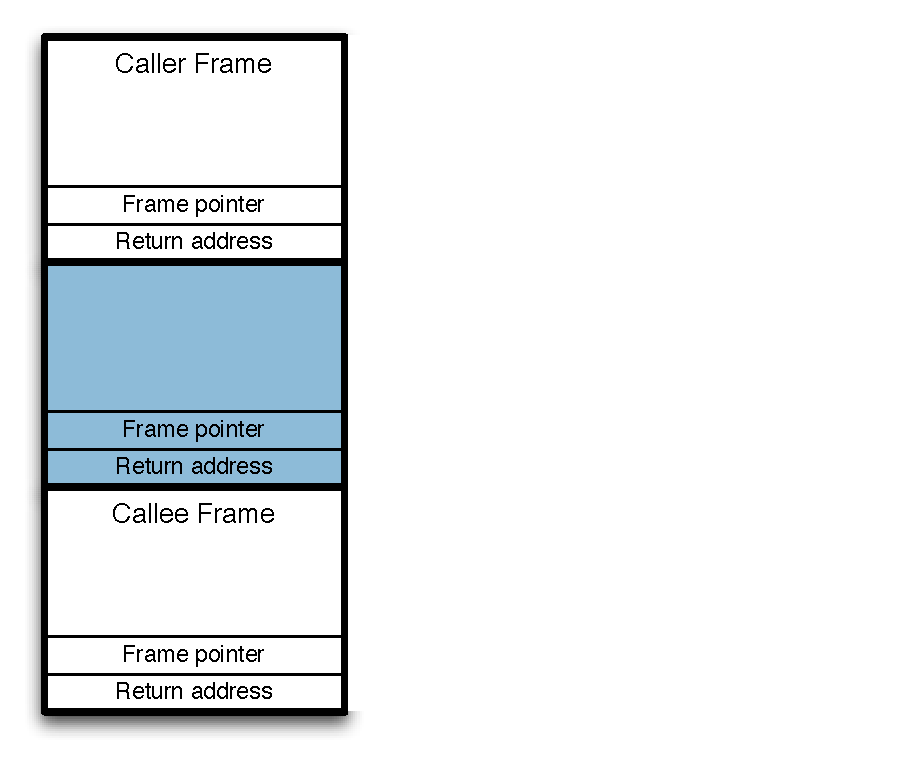
\includegraphics[scale=0.62]{images/stack-smash/stack-frames-overview}\end{center}
\end{frame}

\begin{frame}{Performing On-stack replacement}%{A Sub-title is optional}
\vspace*{-2mm}%
\begin{center}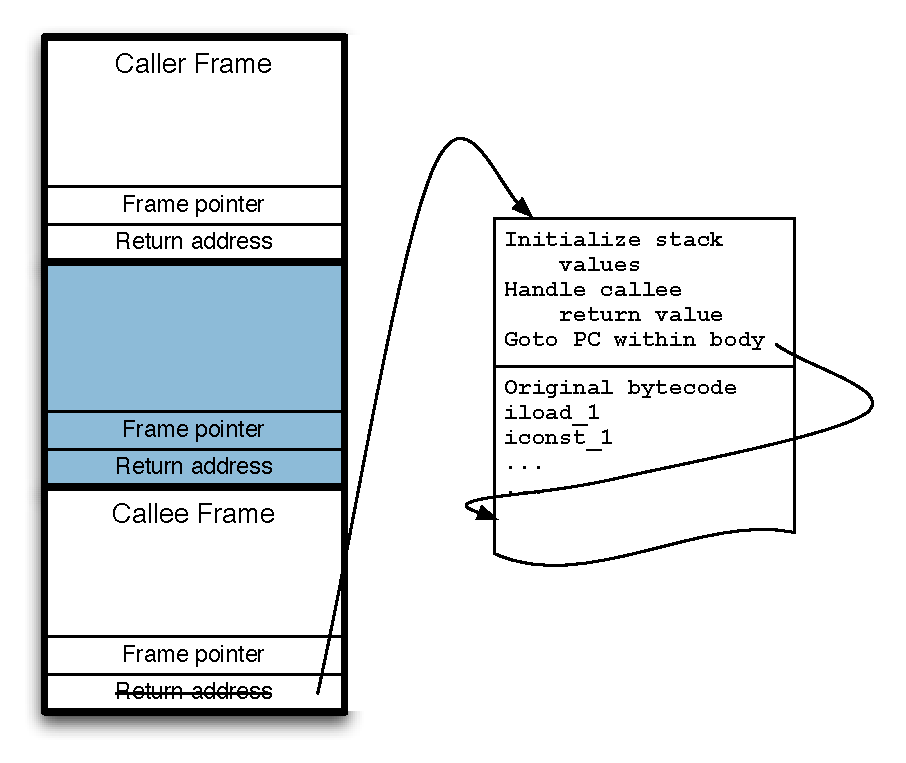
\includegraphics[scale=0.62]{images/stack-smash/osr-overview}\end{center}
\end{frame}

\begin{frame}{Installing return barrier for DSU}%{A Sub-title is optional}
\vspace*{-2mm}%
\begin{center}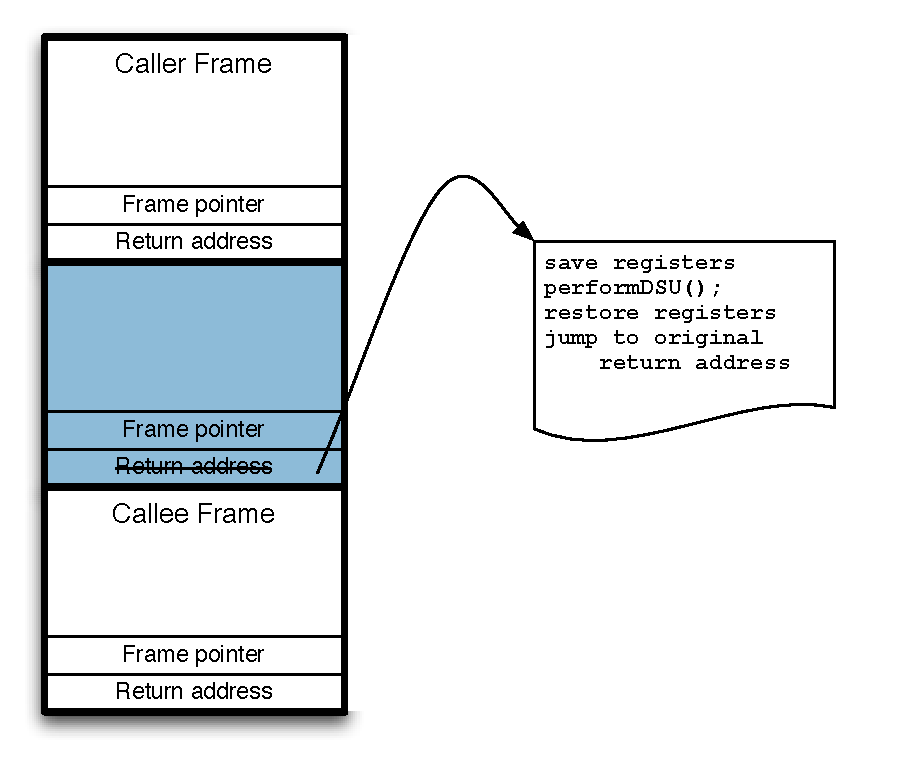
\includegraphics[scale=0.62]{images/stack-smash/return-barrier-overview}\end{center}
\end{frame}

\begin{frame}{Reaching a safe point}%{A Sub-title is optional}
\hspace*{-3mm}
\scalebox{0.44}{%
\uncover<1>{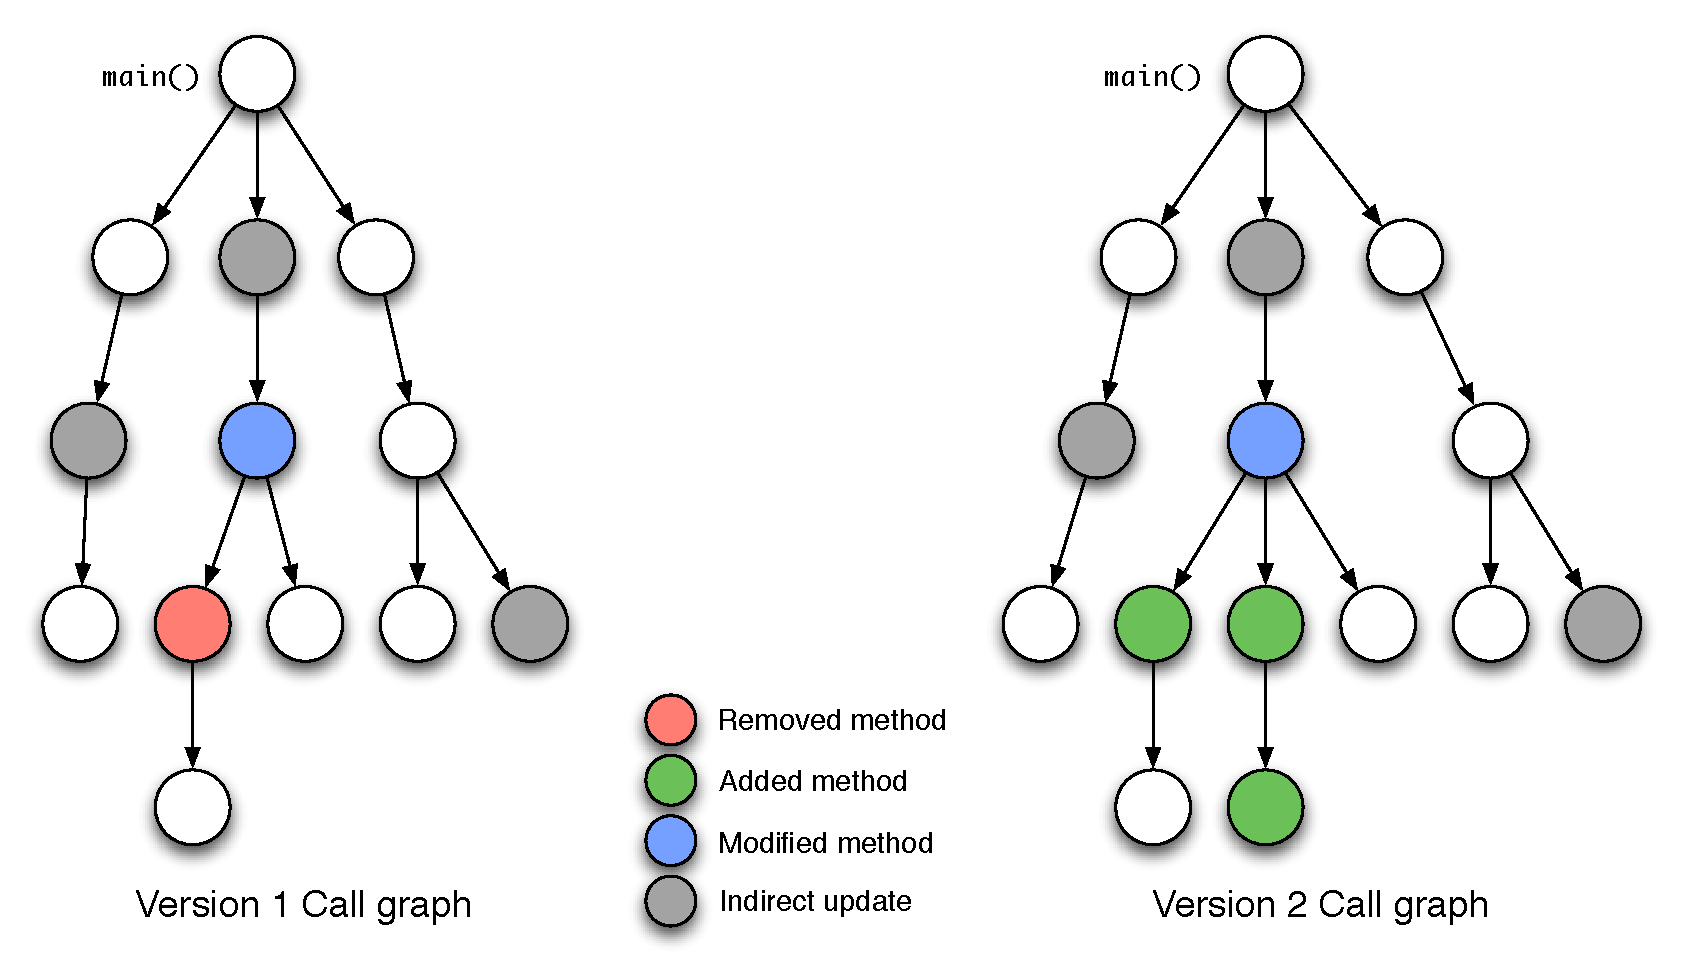
\includegraphics{images/safe-point-call-graph/both-call-graphs-1}}%
\uncover<2>{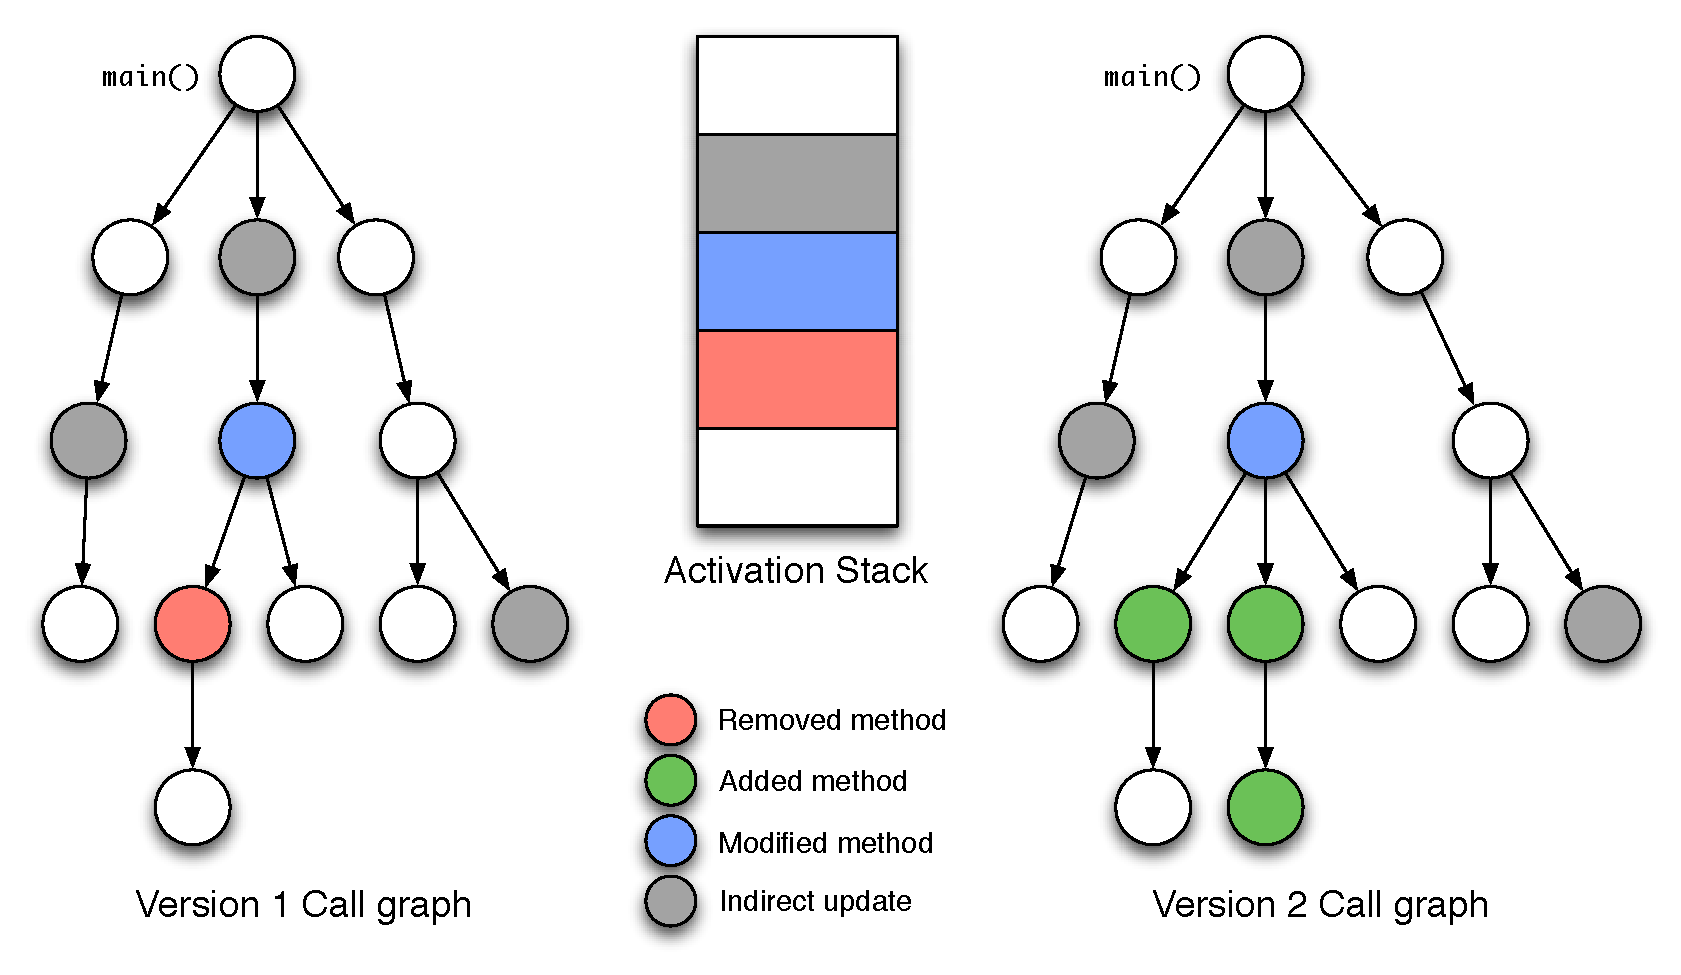
\includegraphics{images/safe-point-call-graph/both-call-graphs-2}}%
\uncover<3>{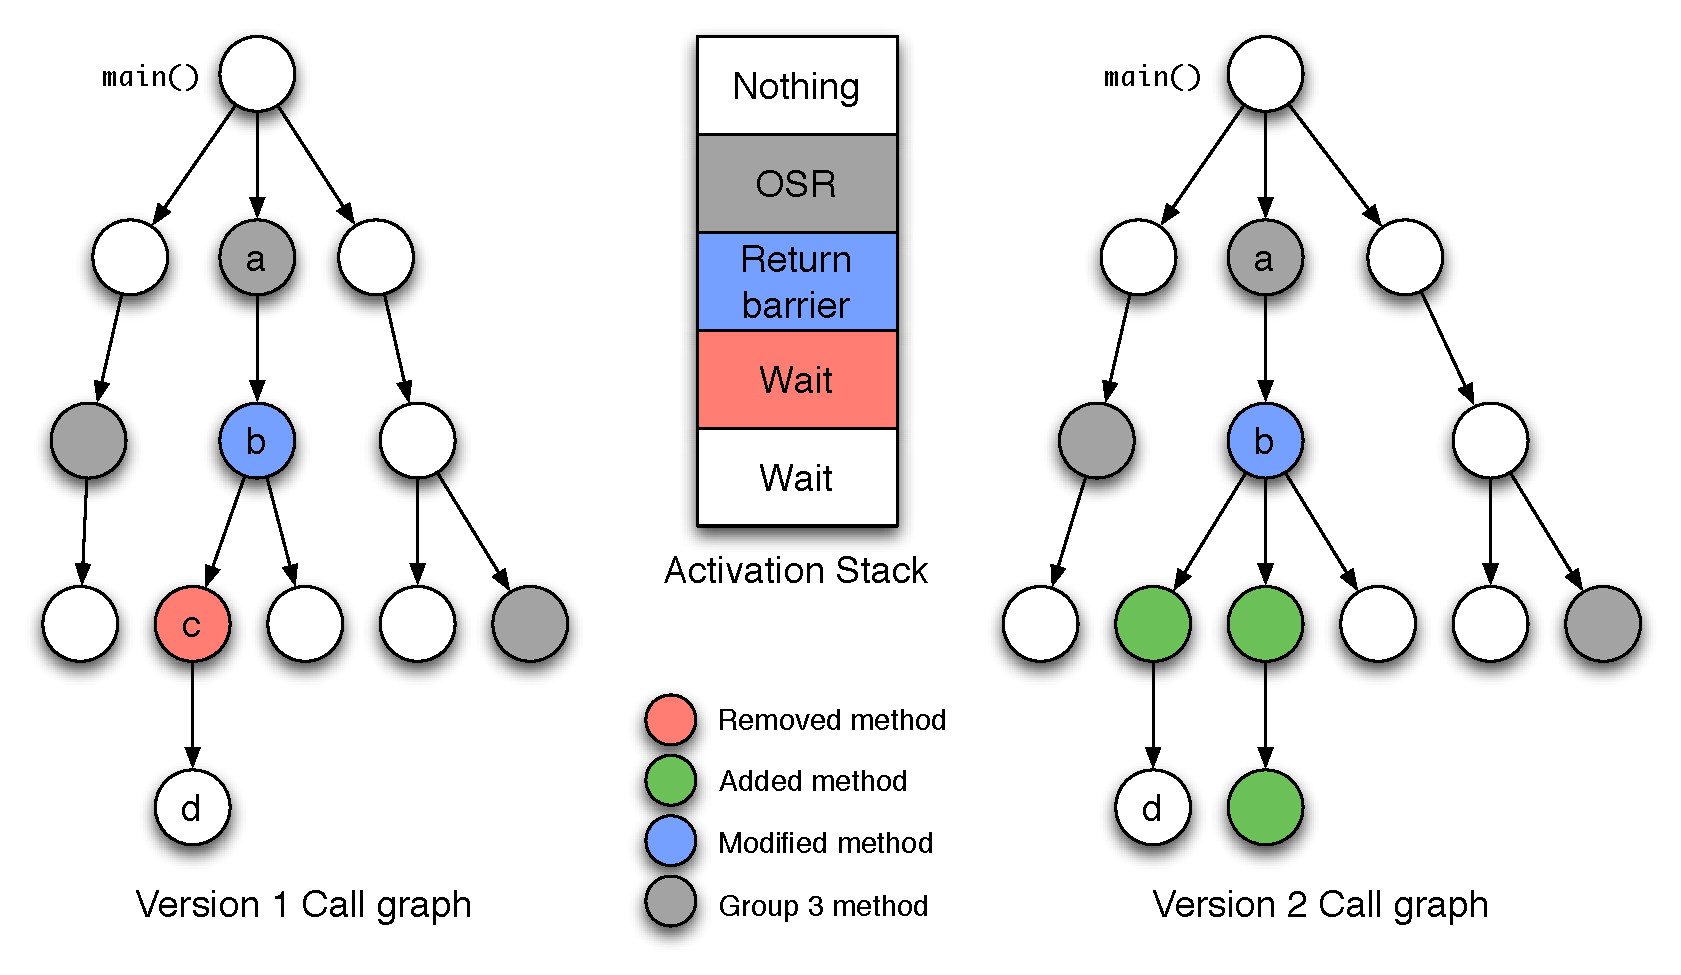
\includegraphics{images/safe-point-call-graph/both-call-graphs-3}}%
}
\end{frame}

% \begin{frame}[c,fragile]{Handling restricted methods}%{A Sub-title is optional}
% \hspace*{-5mm}
% \centering{\scalebox{0.67}{\includegraphics{images/flowchart}}}
% \end{frame}
% 
% \begin{frame}[t,fragile]{On stack replacement in \DSU{}}%{A Sub-title is optional}
% \begin{itemize}
% \item Used in \JikesRVM{} to optimize long running methods
% \item \DSU{} utilizes OSR for DSU
% \item Currently only support baseline-compiled methods
% \item Can OSR any method on stack
% \uncover<2>{
% \item Extract the state of the stack
% \item Construct a new method with a specialized prologue (at the bytecode
% level) that reconstructs the stack
% \item Last instruction of prologue jumps to bytecode where execution should
% resume from
% \item Overwrite the return address to point to the special method
% }
% \end{itemize}
% \end{frame}
% 
% 
% {
% \setbeamercovered{invisible}
% \begin{frame}[t,fragile]{OSR Example}%{A Sub-title is optional}
% \begin{footnotesize}
% \begin{columns}[t]
% 
% \begin{column}{0.4\paperwidth}
% \begin{semiverbatim}
% public class A \{
%   public int foo(int i, B b) \{
%     i = i + 1;
%     i = b.bar(i);
%     i = i + 1;
%     return i;
%   \}
% \}
% \end{semiverbatim}
% 
% \uncover<2-> {
% State: \\
% Thread: \#5 \\
% FP: 0x4ad33e40 \\
% PC: 9 \\
% Locals: i = 5, b = 0x52ae34a0 \\
% Stack vars: S0, S1, ... \\
% }
% \end{column}
% 
% \begin{column}{0.4\paperwidth}
% \begin{semiverbatim}
%  0 iload\_1
%  1 iconst\_1
%  2 iadd
%  3 istore\_1
%  4 aload\_2
%  5 iload\_1
%  6 invokevirtual <B.bar>
%  9 istore\_1
% 10 iload\_1
% 11 iconst\_1
% 12 iadd
% 13 istore\_1
% 14 iload\_1
% 15 ireturn
% \end{semiverbatim}
% \end{column}
% \end{columns}
% \end{footnotesize}
% \end{frame}
% }
% 
% {
% \setbeamercovered{invisible}
% \begin{frame}[t,fragile,shrink=20]{OSR Example}%{A Sub-title is optional}
% \begin{footnotesize}
% \begin{columns}[b]
% 
% \begin{column}{0.4\paperwidth}
% \begin{semiverbatim}
%  0 iload\_1
%  1 iconst\_1
%  2 iadd
%  3 istore\_1
%  4 aload\_2
%  5 iload\_1
%  6 invokevirtual <B.bar>
%  9 istore\_1
% 10 iload\_1
% 11 iconst\_1
% 12 iadd
% 13 istore\_1
% 14 iload\_1
% 15 ireturn
% \end{semiverbatim}
% \end{column}
% 
% \begin{column}{0.4\paperwidth}
% \begin{semiverbatim}
%    ldc 5
%    istore\_0 
%    ldc 0x52ae34a0
%    astore\_1
%    goto 9
%  0 iload\_1
%  1 iconst\_1
%  2 iadd
%  3 istore\_1
%  4 aload\_2
%  5 iload\_1
%  6 invokevirtual <B.bar>
%  9 istore\_1
% 10 iload\_1
% 11 iconst\_1
% 12 iadd
% 13 istore\_1
% 14 iload\_1
% 15 ireturn
% \end{semiverbatim}
% \end{column}
% 
% \end{columns}
% \end{footnotesize}
% \end{frame}
% }


%L  \begin{frame}[t,fragile,label=classload]{Installing new classes}%{A Sub-title is optional}
%L  \JvolveTimeLine{}{}{current}{}{}
%L  The VM maintains Class, Method and Field data structures
%L  % \begin{itemize}
%L  % \item The VM maintains Class, Method and Field data structures
%L  % \item For Method updates: Only load the new method's bytecodes
%L  % \item For Class updates: Rename the old class and load the entire class
%L  % file (equivalent to have loaded two different class)
%L  % \end{itemize}
%L  \begin{center}
%L  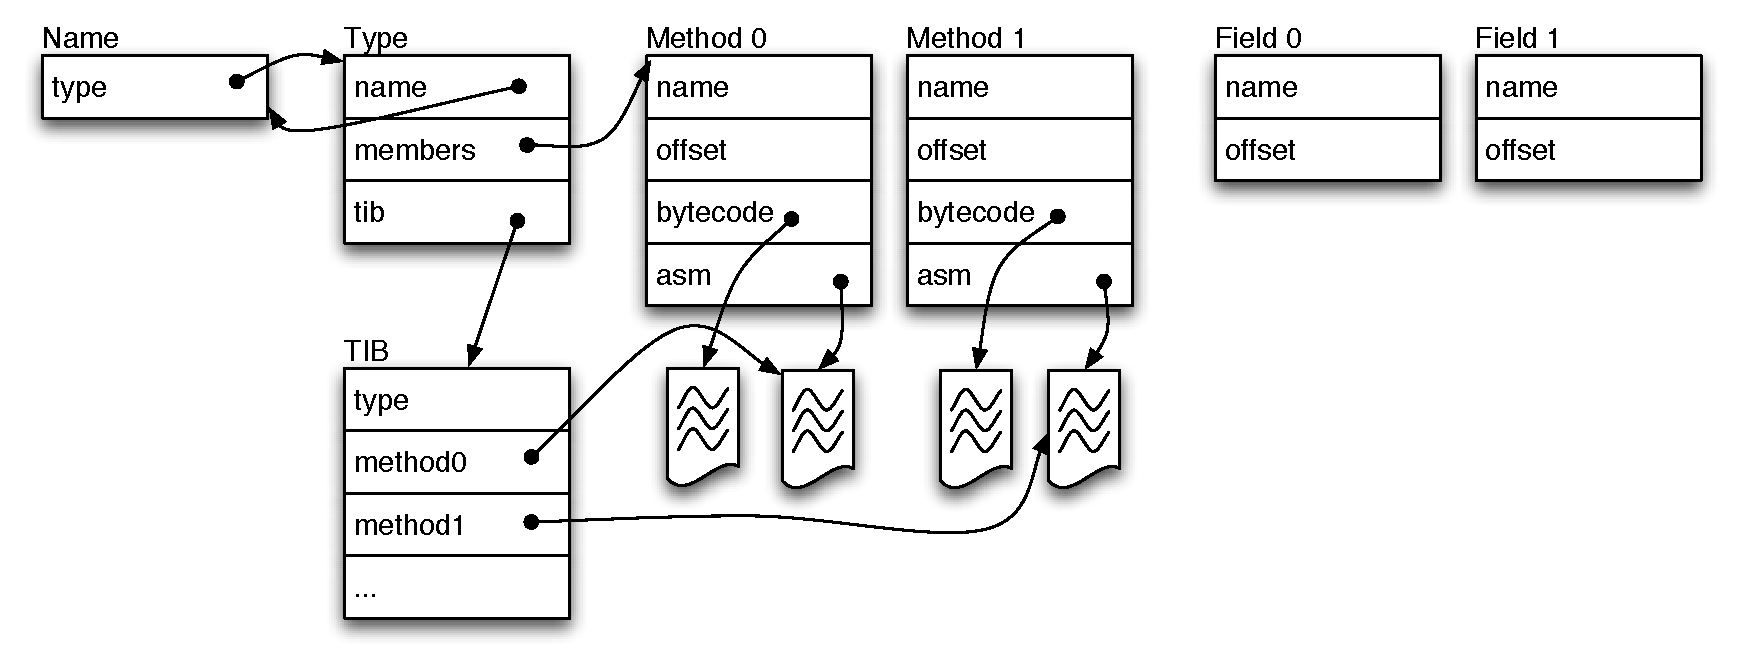
\includegraphics[scale=0.40]{images/vm-meta-data/vm-meta-data}%
%L  \end{center}
%L  \end{frame}
%L
%L  % \ifdraft{}{
%L  % {
\setbeamertemplate{headline}{}
\setbeamertemplate{footline}{}
\setbeamertemplate{navigation symbols}{}
\setbeamercovered{invisible}
\begin{frame}[t,fragile]
\vspace*{-4ex}
\begin{tikzpicture}[auto]

\tikzstyle{title}=[font=\tiny\tt,text width=9mm,minimum height=4.5mm]
\tikzstyle{box}=[font=\tiny\tt,draw, thin,text width=9mm,minimum height=4.5mm,anchor=north west]
% Two rows
\newcommand{\HeaderRow}[2]{% name, content
\node [title] (#1 0) { #2 }; \\
}

\newcommand{\rowsTwo}[3]{% name, row0, row1
\HeaderRow{#1}{#2}
\node [box]   (#1 1) { #3 }; \\
}
% Three rows
\newcommand{\rowsThree}[4]{% name, row0, row1, row2
\rowsTwo{#1}{#2}{#3}
\node [box]   (#1 2) { #4 }; \\
}
% Four rows
\newcommand{\rowsFour}[5]{% name, row0, row1, row2
\rowsThree{#1}{#2}{#3}{#4}
\node [box]   (#1 3) { #5 }; \\
}
% Five rows
\newcommand{\rowsFive}[6]{% name, row0, row1, row2
\rowsFour{#1}{#2}{#3}{#4}{#5}
\node [box]   (#1 4) { #6 }; \\
}

\newcommand{\newRowsTwo}[3]{% name, row0, row1
\HeaderRow{#1}{#2}
\node [box,fill=new color]   (#1 1) { #3 }; \\
}
% Three rows
\newcommand{\newRowsThree}[4]{% name, row0, row1, row2
\newRowsTwo{#1}{#2}{#3}
\node [box,fill=new color]   (#1 2) { #4 }; \\
}
% Four rows
\newcommand{\newRowsFour}[5]{% name, row0, row1, row2
\newRowsThree{#1}{#2}{#3}{#4}
\node [box,fill=new color]   (#1 3) { #5 }; \\
}
% Five rows
\newcommand{\newRowsFive}[6]{% name, row0, row1, row2
\newRowsFour{#1}{#2}{#3}{#4}{#5}
\node [box,fill=new color]   (#1 4) { #6 }; \\
}

\newcommand{\metadataTwo}[4]{% name, position, contents 
\matrix [row sep=-0.4pt,anchor=north west] (#1) at #2 {
\rowsTwo{#1}{#3}{#4}
};}
\newcommand{\metadataThree}[5]{% name, position, contents 
\matrix [row sep=-0.4pt,anchor=north west] (#1) at #2 {
\rowsThree{#1}{#3}{#4}{#5}
};}
\newcommand{\metadataFour}[6]{% name, position, contents 
\matrix [row sep=-0.4pt,anchor=north west] (#1) at #2 {
\rowsFour{#1}{#3}{#4}{#5}{#6}
};}
\newcommand{\metadataFive}[7]{% name, position, contents 
\matrix [row sep=-0.4pt,anchor=north west] (#1) at #2 {
\rowsFive{#1}{#3}{#4}{#5}{#6}{#7}
};}

\newcommand{\newMetadataTwo}[4]{% name, position, contents 
\matrix [row sep=-0.4pt,anchor=north west] (#1) at #2 {
\newRowsTwo{#1}{#3}{#4}
};}
\newcommand{\newMetadataThree}[5]{% name, position, contents 
\matrix [row sep=-0.4pt,anchor=north west] (#1) at #2 {
\newRowsThree{#1}{#3}{#4}{#5}
};}
\newcommand{\newMetadataFour}[6]{% name, position, contents 
\matrix [row sep=-0.4pt,anchor=north west] (#1) at #2 {
\newRowsFour{#1}{#3}{#4}{#5}{#6}
};}
\newcommand{\newMetadataFive}[7]{% name, position, contents 
\matrix [row sep=-0.4pt,anchor=north west] (#1) at #2 {
\newRowsFive{#1}{#3}{#4}{#5}{#6}{#7}
};}

\colorlet{new color}{green!40}
\tikzstyle{line}=[draw, thin, -latex',]
\tikzstyle{every path}=[line]

\begin{scope}
  \metadataTwo{typeref}{(0,-1)}{Name}{type}
  \uncover<4->{ \newMetadataTwo{typerefnew}{(0,0)}{Name}{type} }
  \metadataFour{class}{(2,0)}{Type}{name}{members}{tib}
  \metadataThree{field}{(4,0)}{Field}{name}{offset}
  \node at (5.75,-0.75) {...};
  \metadataFive{method}{(6,0)}{Method}{name}{offset}{bytecode}{asm}
  \metadataFive{tib}{(4,-1.5)}{TIB}{type}{method0}{method1}{...}
  \uncover<-2>{ \node[box,text width=14mm] (bc) at (8,-1)   { 0100100101...  }; }
  \node[box,text width=14mm] (mc) at (8,-2)   { 1010000111... };
  \uncover<2> { \node[box,text width=14mm,fill=new color] (bcnew) at (8,-0.25) { 1100100101... }; }
  \uncover<3->{ \node[box,text width=14mm] (bcnew) at (8,-0.25) { 1100100101... }; }
\end{scope}

\uncover<-3> { \path (typeref 1.east) to [out=0,in=180] (class 1.north west); }
\uncover<-3> { \path (class 1.west)   to [out=180,in=0] (typeref 1.south east); }
\uncover<4-> { \path (typerefnew 1.east) to [out=0,in=180] (class 1.north west); }
\uncover<4-> { \path (class 1.west)   to [out=180,in=0] (typerefnew 1.south east); }
\path (class 2.east)         to [out=0,in=180]   (field 1.north west);
\path (class 3.east)         to [out=0,in=135]   (tib 1.north west);
\path (tib 1.west)           to [out=180,in=315] (class 3.south);
\path (tib 2.east)           to [out=0,in=225]   (mc.south west);
\path (method 4.east)        to                  (mc.north west);
\uncover<1>  { \path (method 3.east)        to   (bc.north west);    }
\uncover<2-> { \path (method 3.east)        to   (bcnew.north west); }

\uncover<5->{
\begin{scope}[yshift=-4.5cm]
  \newMetadataFour{class1}{(2,0)}{Type}{name}{members}{tib}
  \newMetadataThree{field1}{(4,0)}{Field}{name}{offset}
  \node at (5.75,-0.75) {...};
  \newMetadataFive{method1}{(6,0)}{Method}{name}{offset}{bytecode}{asm}
  \newMetadataFive{tib1}{(4,-1.5)}{TIB}{type}{method0}{method1}{...}
  \node[box,text width=14mm,fill=new color] (bc1) at (8,-1) { 0100100101... };
  \node[box,text width=14mm,fill=new color] (mc1) at (8,-2) { 1010000111... };
\end{scope}
  \path (class1 2.east)         to [out=0,in=180]   (field1 1.north west);
  \path (class1 3.east)         to [out=0,in=135]   (tib1 1.north west);
  \path (tib1 2.east)           to [out=0,in=225]   (mc1.south west);
  \path (tib1 1.west)           to [out=180,in=315] (class1 3.south);
  \path (method1 3.east)        to                  (bc1.north west);
  \path (method1 4.east)        to                  (mc1.north west);
  \path (class1 1.north west)   to                  (typeref 1.south east);
  \path (typeref 1.south)       to [out=285,in=180] (class1 1.west);
}

\end{tikzpicture}
\end{frame}
}

%L  % }
%L
%L  \begin{frame}{Updating a method}%{A Sub-title is optional}
%L  \vspace*{-1mm}%
%L  \begin{center}
%L  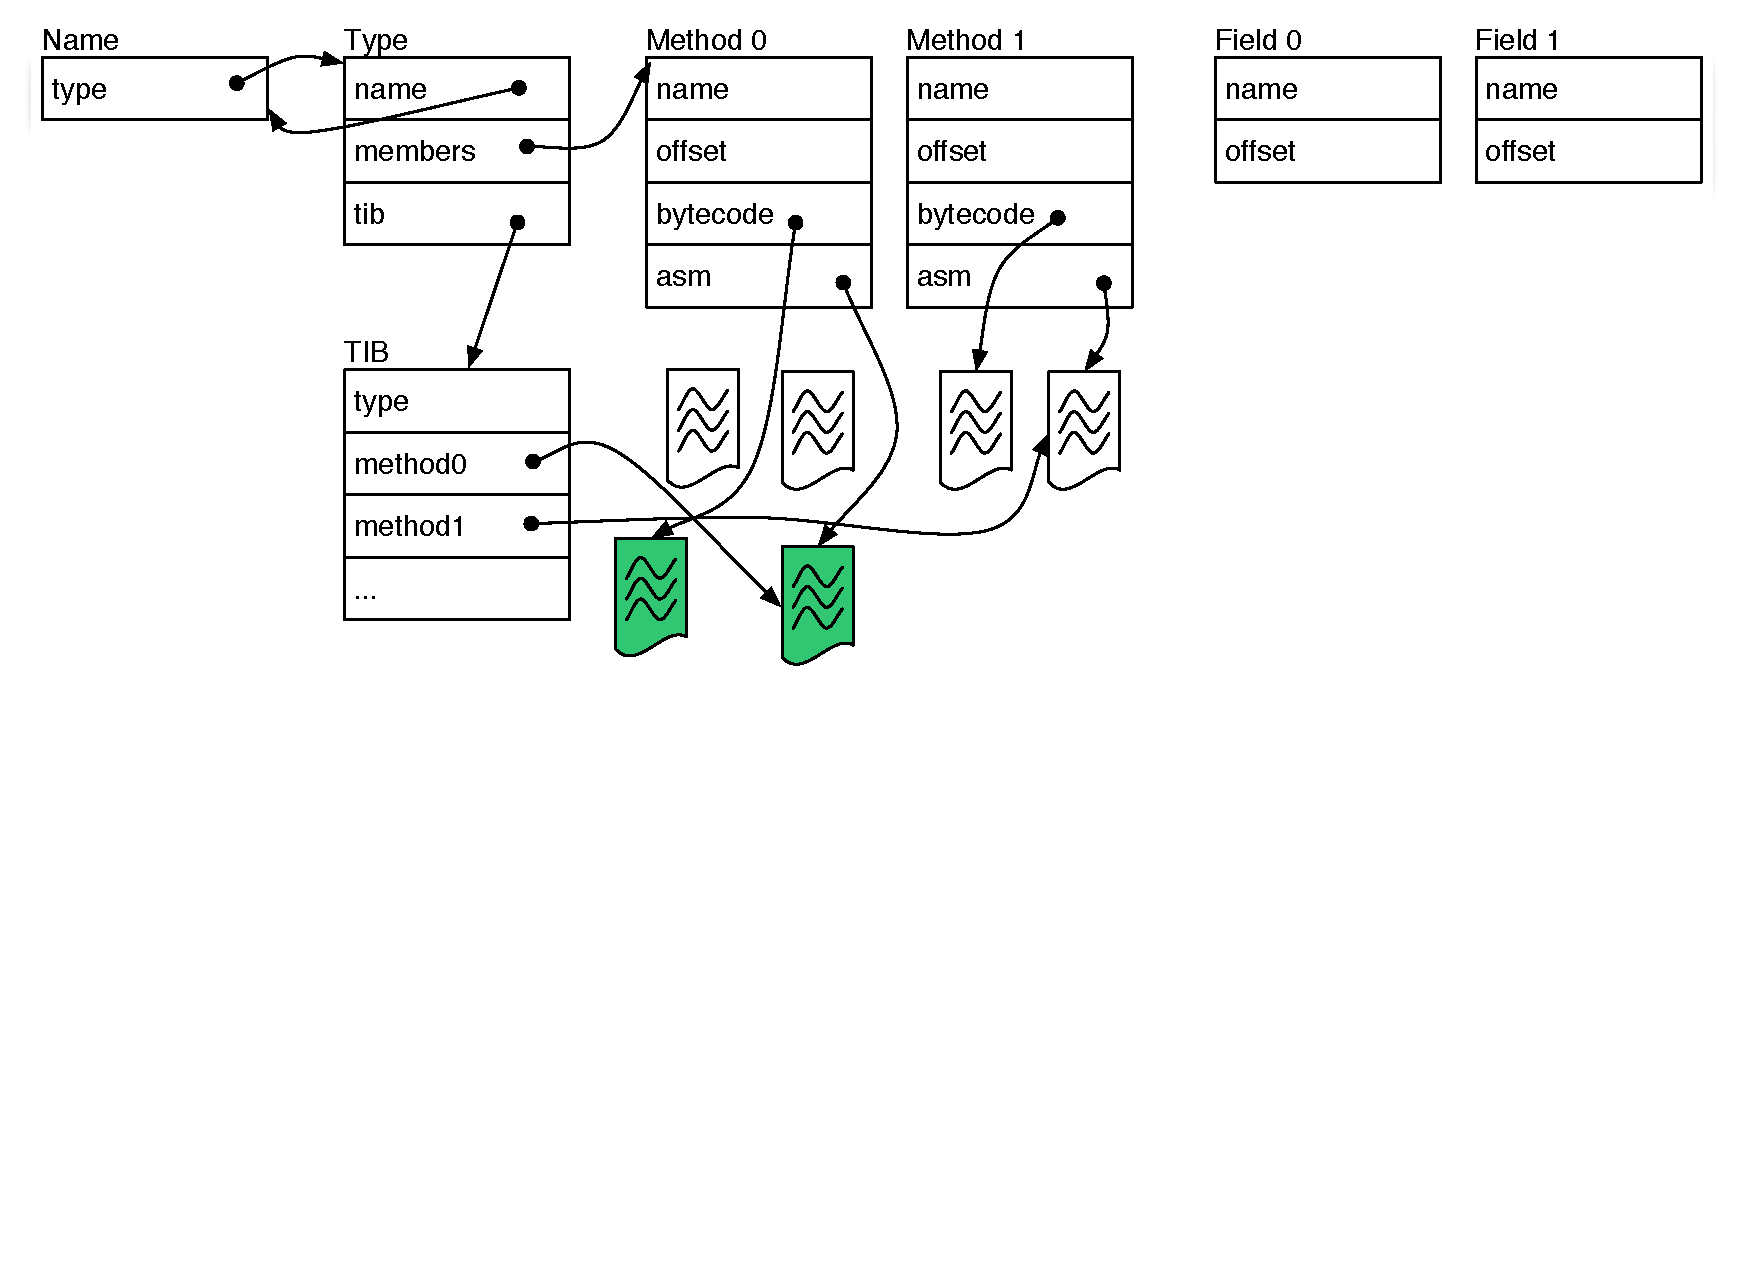
\includegraphics[scale=0.36]{images/vm-meta-data/vm-meta-data-updated-method}%
%L  \end{center}
%L  \end{frame}
%L
%L  \begin{frame}{Updating a class}%{A Sub-title is optional}
%L  \vspace*{-1mm}%
%L  \begin{center}
%L  \includegraphics[scale=0.36]<1>{images/vm-meta-data/vm-meta-data-renamed-class}%
%L  \includegraphics[scale=0.36]<2>{images/vm-meta-data/vm-meta-data-updated-class}%
%L  \end{center}
%L  \end{frame}

\begin{frame}{Update code}%{A Sub-title is optional}
\vspace*{-3mm}%
\begin{center}%
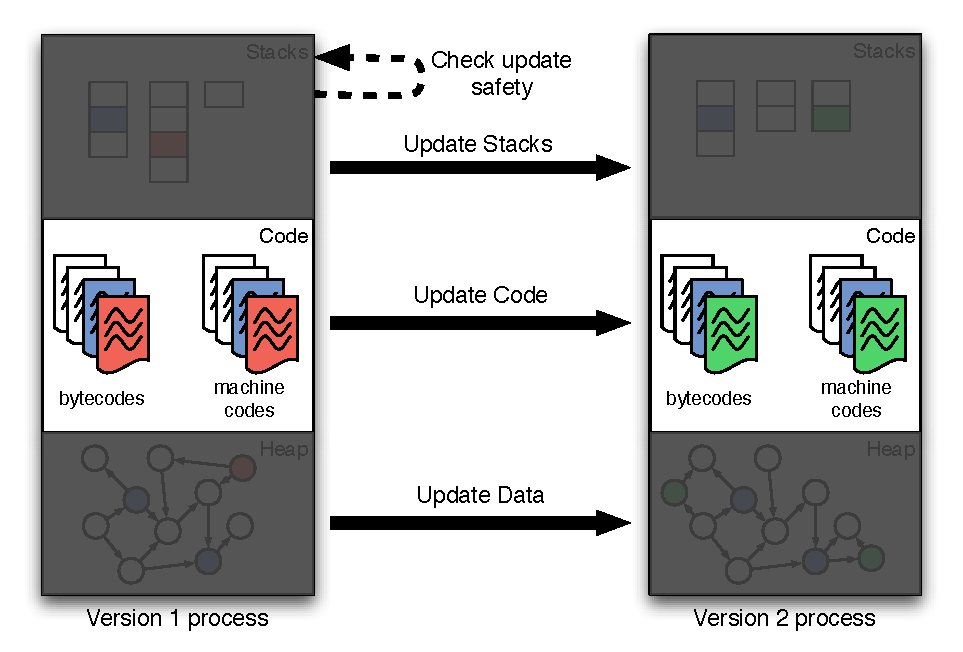
\includegraphics[scale=0.73]{images/process-state/both-process-state-highlight-code}%
\end{center}%
\end{frame}

\begin{frame}{Update code}%{A Sub-title is optional}
\begin{itemize}
\item Modify class loader to recognize new versions of classes
\item Install new versions of classes and methods
\item Rely on Just-in-time Compiler to compile new versions of methods on
demand
\item Extend On-stack replacement to update active methods
\end{itemize}
\end{frame}

% \begin{frame}{Updating a method}%{A Sub-title is optional}
% \vspace*{-1mm}%
% \begin{center}
% 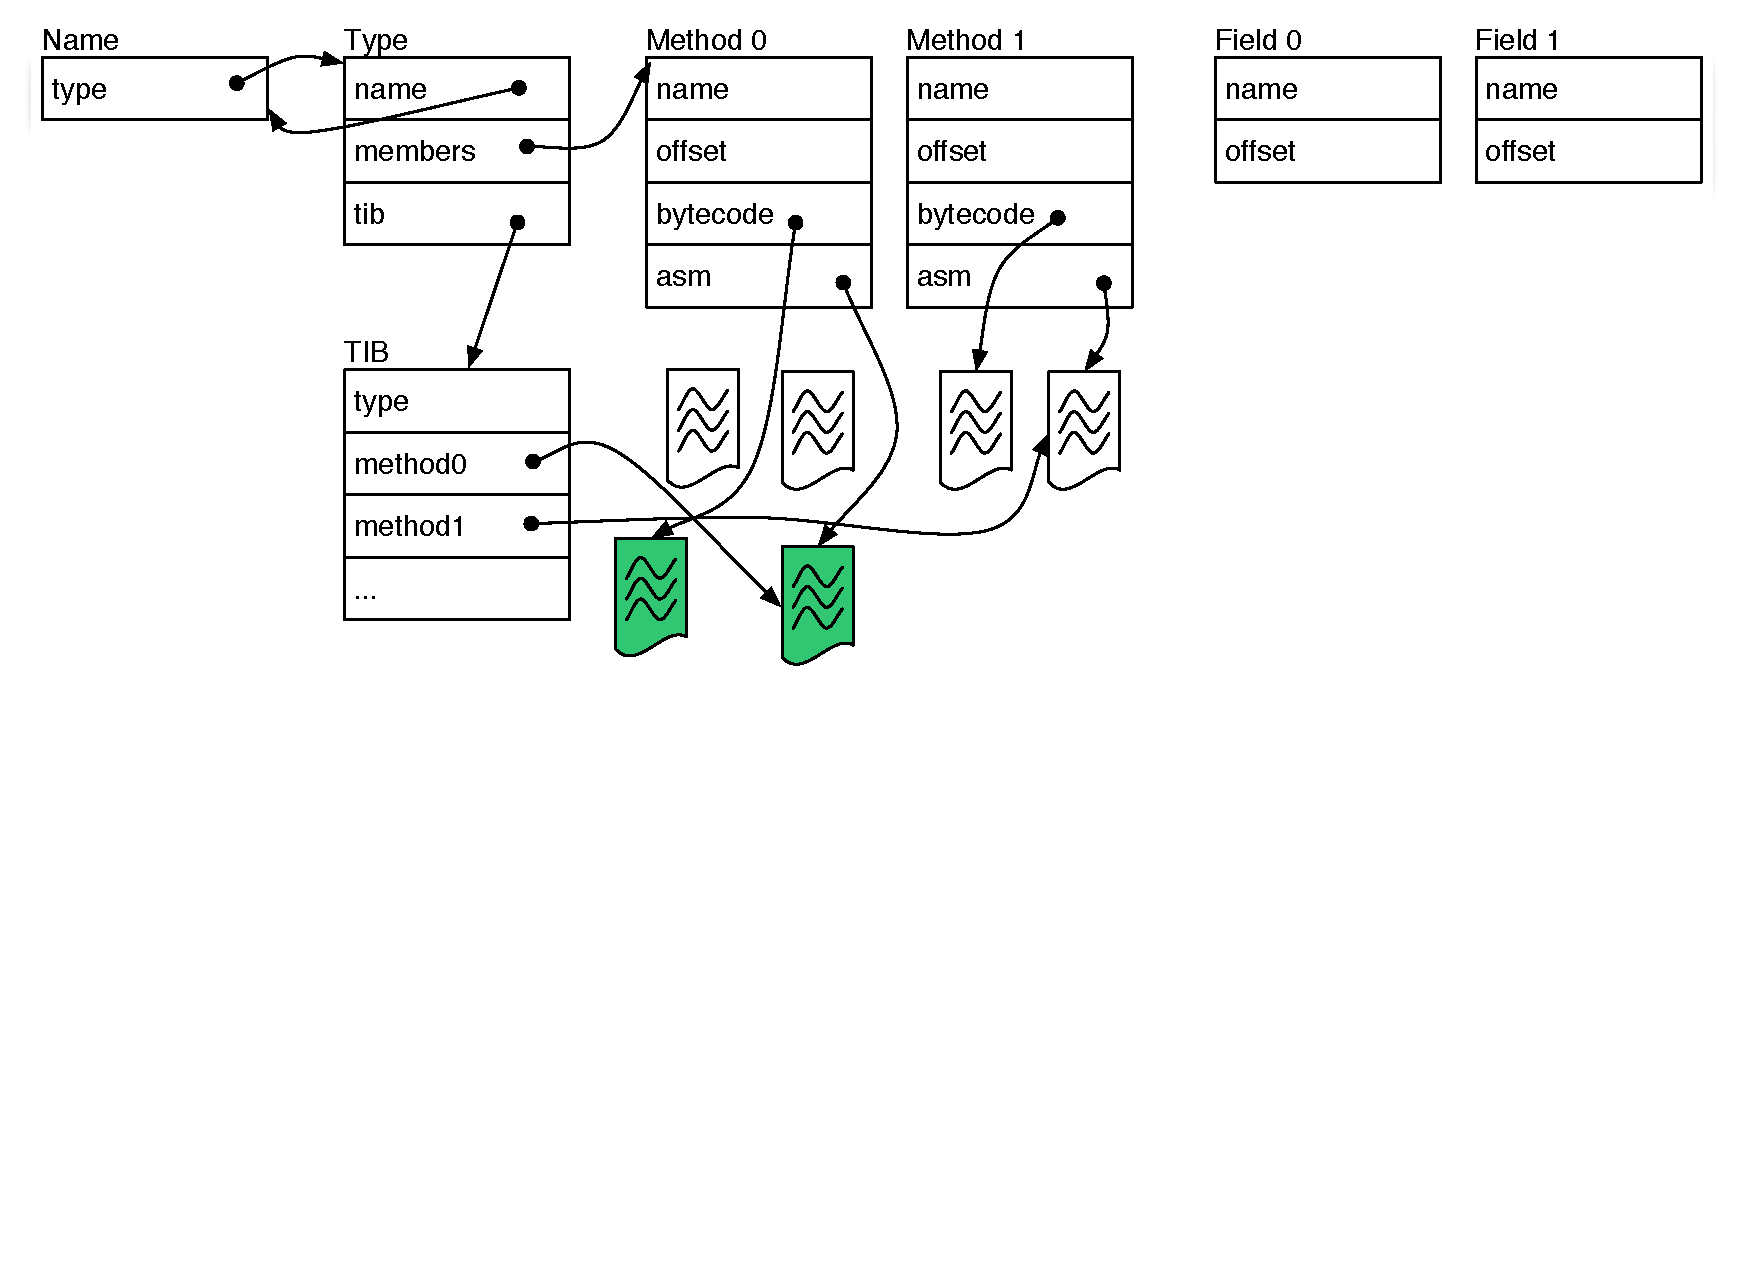
\includegraphics[scale=0.36]{images/vm-meta-data/vm-meta-data-updated-method}%
% \end{center}
% \end{frame}
% 
% \begin{frame}{Updating a class}%{A Sub-title is optional}
% \vspace*{-1mm}%
% \begin{center}
% \only<1>{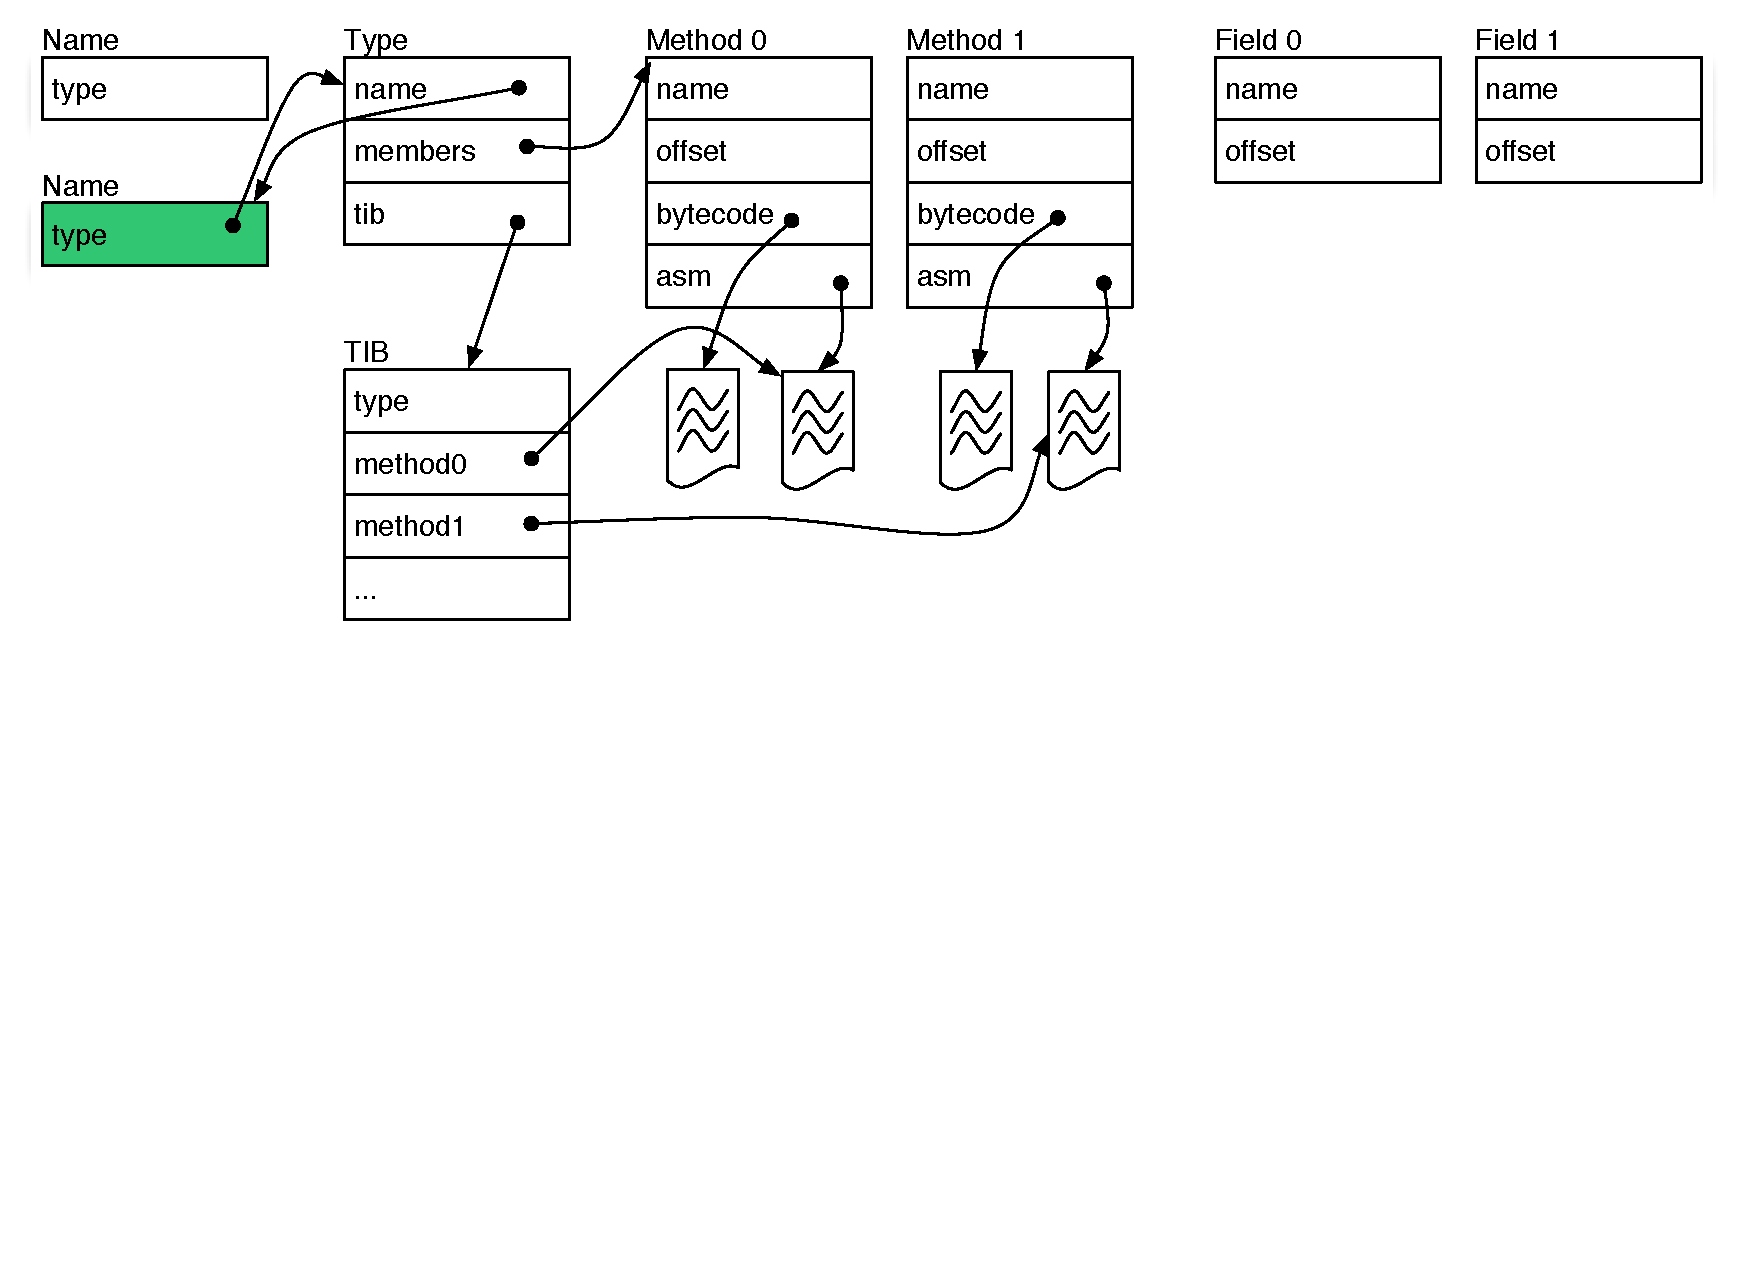
\includegraphics[scale=0.36]{images/vm-meta-data/vm-meta-data-renamed-class}}%
% \only<2>{\includegraphics[scale=0.36]{images/vm-meta-data/vm-meta-data-updated-class}}%
% \end{center}
% \end{frame}

\begin{frame}{Update data}%{A Sub-title is optional}
\vspace*{-3mm}%
\begin{center}%
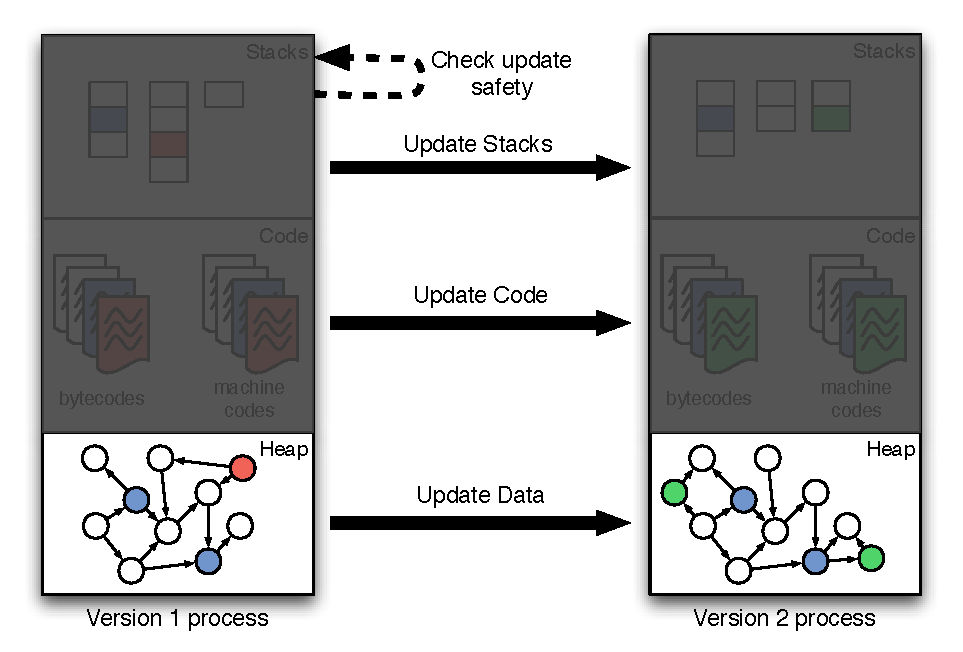
\includegraphics[scale=0.73]{images/process-state/both-process-state-highlight-heap}%
\end{center}%
\end{frame}

% \newcommand{\ExampleCodeSize}{footnotesize}

% \newcommand{\removed}[1]{\textcolor{red}{- #1}}
% \newcommand{\addedxx}[1]{\textcolor{OliveGreen}{+ #1}}

\begin{frame}[fragile,shrink=5]{Example of an update (JavaEmailServer)}%{A Sub-title is optional}
\begin{\ExampleCodeSize}
\begin{semiverbatim}
  public class User \{
    private final String username, domain, password;
\removed{  private String[] forwardAddresses;}
\addedxx{  private EmailAddress[] forwardAddresses;}
    public User(...) \{...\}
    public String[] getForwardedAddresses() \{...\}

    public void setForwardedAddresses(String[] f) \{...\}

  \}

  public class ConfigurationManager \{
    private User loadUser(...) \{
       ...
       User user = new User(...);
       String[] f = ...;

       user.setForwardedAddresses(f);
       return user;
    \}
  \}
\end{semiverbatim}
\end{\ExampleCodeSize}
\end{frame}


% \begin{frame}[fragile,shrink=5]{Example of an update (JavaEmailServer)}%{A Sub-title is optional}
% \begin{\ExampleCodeSize}
% \begin{semiverbatim}
% public class User \{
%   private String username, domain, password;
%   private \sout{String[]} EmailAddress[] forwardAddresses;
%   public \sout{String[]} EmailAddress[] getForwardedAddresses() \{...\}
%   public void setForwardedAddresses(\sout{String[]} EmailAddress[] f) \{...\}
% \}
% 
% public class ConfigurationManager \{
%   private User loadUser(...) \{
%      ...
%      User user = new User(...);
%      \sout{String[]} EmailAddress[] f = ...;
%      user.setForwardedAddresses(f);
%      return user;
%   \}
% \}
% 
% \end{semiverbatim}
% \end{\ExampleCodeSize}
% \end{frame}

\begin{frame}[fragile,shrink=5]{Example of an update (JavaEmailServer)}%{A Sub-title is optional}
\begin{\ExampleCodeSize}
\begin{semiverbatim}
  public class User \{
    private final String username, domain, password;
\removed{  private String[] forwardAddresses;}
\addedxx{  private EmailAddress[] forwardAddresses;}
    public User(...) \{...\}
\removed{  public String[] getForwardedAddresses() \{...\}}
\addedxx{  public EmailAddress[] getForwardedAddresses() \{...\}}
\removed{  public void setForwardedAddresses(String[] f) \{...\}}
\addedxx{  public void setForwardedAddresses(EmailAddress[] f) \{...\}}
  \}

  public class ConfigurationManager \{
    private User loadUser(...) \{
       ...
       User user = new User(...);
\removed{     String[] f = ...;}
\addedxx{     EmailAddress[] f = ...;}
       user.setForwardedAddresses(f);
       return user;
    \}
  \}
\end{semiverbatim}
\end{\ExampleCodeSize}
\end{frame}

\begin{frame}[fragile,shrink=5]{Example of an update (JavaEmailServer)}%{A Sub-title is optional}
\mode<beamer> {
\begin{textblock*}{46mm}[0,0](79mm,20mm)
\begin{block}{}
Stub generated by UPT for the old version
\end{block}
\end{textblock*}
\only<1>{
\begin{textblock*}{46mm}[0,0](79mm,48mm)
\begin{block}{}
Default transformer copies old fields, initializes new ones to
\texttt{null}
\end{block}
\end{textblock*}}
}
\begin{small}
\begin{semiverbatim}
public class v131_User \{
  private final String username, domain, password;
  private String[] forwardAddresses;
\}
public class JvolveTransformers \{
 ...
 public static void jvolveClass(User unused) \{\}
 public static void jvolveObject(User to, v131_User from) \{
    to.username = from.username;
    to.domain = from.domain;
    to.password = from.password;
    // to.forwardAddresses = null;
    \uncover<2>{int len = from.forwardAddresses.length;
    to.forwardAddresses = new EmailAddress[len];
    for (int i = 0; i < len; i++) \{
      to.forwardAddresses[i] =
        new EmailAddress(from.forwardAddresses[i]);
}\}\}\}

\end{semiverbatim}
\end{small}
\end{frame}



\begin{frame}[t]{Transforming objects in the GC}%{A Sub-title is optional}
\vspace*{-6ex}
\begin{center}
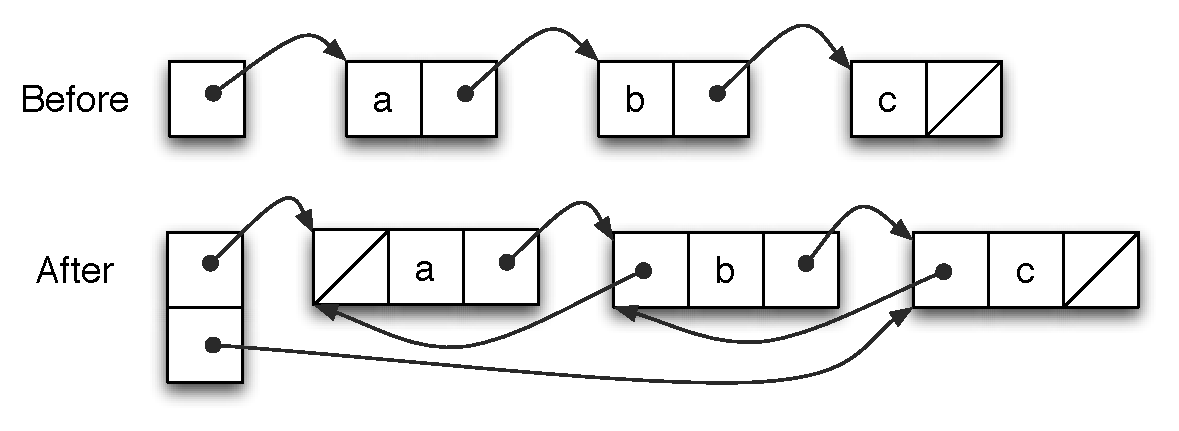
\includegraphics[scale=0.6]{images/singly-doubly/linked-lists-without-gc}%
\end{center}
Happens in two steps \\
\begin{itemize}
\item Garbage collector creates an additional empty copy for updated objects
\item Walk through and transform all these objects
\end{itemize}
% \begin{itemize}
% % \item Supported on top of a semi-space copying collector
% % \item Regular GC
% %   \begin{itemize}
% %   \item Copies all live objects to ``to'' space
% %   \end{itemize}
% \item Jvolve's GC
%   \begin{itemize}
%   \item Built on top of a semi-space copying collector
%   \item Copies all live objects to ``to'' space
%   \item For updated objects, allocate an empty object in ``to'' space
%   \item Forwarding pointers and object pointers point to these empty
%   objects
%   \item After GC, walk through all updated objects and run their
%   transformation functions
%   \end{itemize}
% \end{itemize}
\end{frame}

% \ifdraft{}{
% 
%%%%%%%%%%%%%%%%%%%%%%%%%%%%%%%%%%%%%%%%%%%%%%%%%%%%%%%%%%%%%%%%%%%%%%%%
% Colors
\colorlet{black object color}{black!60}
\colorlet{grey object color}{black!20}
\colorlet{forwarding pointer color}{structure.fg!40}
\colorlet{dsu v0 color}{blue!60}
\colorlet{dsu v1 empty color}{blue!20}
\colorlet{dsu forwarding pointer color}{forwarding pointer color!50!dsu v0 color}
%%%%%%%%%%%%%%%%%%%%%%%%%%%%%%%%%%%%%%%%%%%%%%%%%%%%%%%%%%%%%%%%%%%%%%%%

%%%%%%%%%%%%%%%%%%%%%%%%%%%%%%%%%%%%%%%%%%%%%%%%%%%%%%%%%%%%%%%%%%%%%%%%
% Define the style for each field of the object
\newlength{\drawthickness}
\setlength{\drawthickness}{0.6pt}
\newlength{\fielddimension}
\setlength{\fielddimension}{5mm}
\tikzstyle{field}=[
    rectangle,
    draw=black,
    line width=\drawthickness,
    minimum width=\fielddimension,
    minimum height=\fielddimension,
    inner sep=0pt,
    font=\tiny,
]
\tikzstyle{new space grey field}=[field,fill=grey object color]
\tikzstyle{new space black field}=[field,fill=black object color]
\tikzstyle{dsu v0 field}=[field,fill=dsu v0 color]
\tikzstyle{dsu v1 empty field}=[field,fill=dsu v1 empty color]
%%%%%%%%%%%%%%%%%%%%%%%%%%%%%%%%%%%%%%%%%%%%%%%%%%%%%%%%%%%%%%%%%%%%%%%%

%%%%%%%%%%%%%%%%%%%%%%%%%%%%%%%%%%%%%%%%%%%%%%%%%%%%%%%%%%%%%%%%%%%%%%%%
% Define the style for each object
\tikzstyle{object}=[
    column sep=-\drawthickness,
    nodes=field,
    inner sep=0pt,
]
\tikzstyle{new space grey object}=[object,nodes=new space grey field]
\tikzstyle{new space black object}=[object,nodes=new space black field]
\tikzstyle{dsu v0 object}=[object,nodes=dsu v0 field]
\tikzstyle{dsu v1 empty object}=[object,nodes=dsu v1 empty field]
%%%%%%%%%%%%%%%%%%%%%%%%%%%%%%%%%%%%%%%%%%%%%%%%%%%%%%%%%%%%%%%%%%%%%%%%

%%%%%%%%%%%%%%%%%%%%%%%%%%%%%%%%%%%%%%%%%%%%%%%%%%%%%%%%%%%%%%%%%%%%%%%%
% Style for arrows
\tikzstyle{regular}=[-to,draw]
\tikzstyle{transparent}=[-to,draw=black!15!bg]
%%%%%%%%%%%%%%%%%%%%%%%%%%%%%%%%%%%%%%%%%%%%%%%%%%%%%%%%%%%%%%%%%%%%%%%%

%%%%%%%%%%%%%%%%%%%%%%%%%%%%%%%%%%%%%%%%%%%%%%%%%%%%%%%%%%%%%%%%%%%%%%%%
% Define a macro for creating an object with two fields
\newcommand{\twoFieldsObject}[3]{% name, position, object style
\matrix[#3,ampersand replacement=\&] (#1) at #2 {
  \node (#1 0) {}; \& \node (#1 1) {}; \\
};}
\newcommand{\fourFieldsObject}[3]{% name, position, object style
\matrix[#3,ampersand replacement=\&] (#1) at #2 {
  \node (#1 0) {}; \& \node (#1 1) {}; \& \node (#1 2) {}; \& \node (#1 3) {}; \\
};}


% Command to write a label next to an object
\newcommand{\labelObject}[4]{% label text, object name, label position, label anchor
\draw (#2.#3) node[anchor=#4,inner sep=0.5pt,font=\tiny] {#1};}
\newcommand{\oldSpaceLabelObject}[2]{% label text, object name
\labelObject{#1}{#2}{north west}{north east}}
\newcommand{\newSpaceLabelObject}[2]{% label text, object name
\labelObject{#1}{#2}{150}{south west}}

\newcommand{\oldSpaceObject}[3][object]{% object style, name, position
\twoFieldsObject{#2}{#3}{#1}\oldSpaceLabelObject{#2}{#2}}
\newcommand{\dsuOldSpaceVersionZeroObject}[2]{% name, location
\twoFieldsObject{#1}{#2}{dsu v0 object}\oldSpaceLabelObject{#1 $v_0$}{#1}}
\newcommand{\dsuOldSpaceVersionOneObject}[2]{% name, location
\fourFieldsObject{#1 v1}{#2}{dsu v1 empty object}\oldSpaceLabelObject{#1 $v_1$}{#1 v1}}

\newcommand{\newSpaceObject}[4][]{% extra name, name, position, object style
\twoFieldsObject{#2}{#3}{#4}\newSpaceLabelObject{#2#1}{#2}}
\newcommand{\newSpaceVersionOneEmptyObject}[2]{% name, position
\fourFieldsObject{#1 v1}{#2}{dsu v1 empty object}\labelObject{#1 $v_1$}{#1 v1}{165}{south west}}
\newcommand{\newSpaceGreyObject}[2]{% name, position
\newSpaceObject{#1}{#2}{new space grey object}}
\newcommand{\newSpaceBlackObject}[2]{% name, position
\newSpaceObject{#1}{#2}{new space black object}}
\newcommand{\dsuNewSpaceGreyObject}[2]{% name, position
\newSpaceObject[\ $v_0$]{#1}{#2}{new space grey object}}
\newcommand{\dsuNewSpaceBlackObject}[2]{% name, position
\newSpaceObject[\ $v_0$]{#1}{#2}{new space black object}}

\newcommand{\forwardingPointer}[1]{% name
\node[field,minimum width=2\fielddimension,fill=forwarding pointer color] at (#1.center) {#1'};
}
\newcommand{\dsuForwardingPointer}[1]{% name
\node[field,minimum width=2\fielddimension,fill=dsu forwarding pointer color] at (#1.center) {#1' $v_1$};
}
%%%%%%%%%%%%%%%%%%%%%%%%%%%%%%%%%%%%%%%%%%%%%%%%%%%%%%%%%%%%%%%%%%%%%%%%

%%%%%%%%%%%%%%%%%%%%%%%%%%%%%%%%%%%%%%%%%%%%%%%%%%%%%%%%%%%%%%%%%%%%%%%%
% Define coordinates of the various objects
\newcommand{\objectRoot}{(-3,0.8)}
\newcommand{\objectA}{(0,0)}
\newcommand{\objectB}{(-2,-1)}
\newcommand{\objectC}{(2,-1)}
\newcommand{\objectD}{(-3,-2)}
\newcommand{\objectE}{(-1,-2)}
\newcommand{\objectF}{(1,-2)}
\newcommand{\objectG}{(3,-2)}

\newcommand{\objectAprime}{(-3.5,0.25)}
\newcommand{\objectBprime}{(-2.5,0.25)}
\newcommand{\objectCprime}{(-1.5,0.25)}
\newcommand{\objectDprime}{(-0.5,0.25)}
\newcommand{\objectEprime}{(+0.5,0.25)}
\newcommand{\objectFprime}{(+1.5,0.25)}
\newcommand{\objectGprime}{(+2.5,0.25)}

% old space
\newcommand{\objectCVersionOne}{(2.5,0)}
\newcommand{\objectFVersionOne}{(1,-3)}
% new space
\newcommand{\objectCprimeVersionOne}{(-3,-1.75)}
\newcommand{\objectFprimeVersionOne}{(-0.75,-1.75)}
%%%%%%%%%%%%%%%%%%%%%%%%%%%%%%%%%%%%%%%%%%%%%%%%%%%%%%%%%%%%%%%%%%%%%%%%

% vim:tw=0:nospell

% % 
% The various steps of the animation are
% Slide 1: Show all objects
% Slide 2: A is copied
% Slide 3: A is scanned; B, C are copied
% Slide 4: A, B are scanned; C, D, E are copied
% Slide 5: A, B, C are scanned; D, E, F, G are copied
% Slide 6: A-D are scanned
% Slide 7: A-E are scanned
% Slide 8: A-F are scanned
% Slide 9: A-G are scanned
{
\begin{frame}[fragile]{Semi-space copying collector}%{A Sub-title is optional}
\setbeamercovered{invisible}
\begin{columns}[t]
\begin{column}[T]{0.67\paperwidth}
\begin{tikzpicture}
\begin{scope}
  % objects
  \uncover<1>{       \node[field] (root) at \objectRoot {root};                        }
  \uncover<2->{      \node[new space black field] (root) at \objectRoot {root};        }
                     \oldSpaceObject{A}{\objectA}
                     \oldSpaceObject{B}{\objectB}
                     \oldSpaceObject{C}{\objectC}
                     \oldSpaceObject{D}{\objectD}
                     \oldSpaceObject{E}{\objectE}
                     \oldSpaceObject{F}{\objectF}
                     \oldSpaceObject{G}{\objectG}
  % forwarding pointers
  \uncover<2->{      \forwardingPointer{A}                             }
  \uncover<3->{      \forwardingPointer{B}
                     \forwardingPointer{C}                             }
  \uncover<4->{      \forwardingPointer{D}
                     \forwardingPointer{E}                             }
  \uncover<5->{      \forwardingPointer{F}
                     \forwardingPointer{G}                             }
  % pointer arrows
  \uncover<1>   {    \path[regular]     (root.east)  to [out=330,in=120] (A.140)    ;          }
  \uncover<1>   {    \path[regular]     (A 0.center) to                (B.90)     ;            }
  \uncover<1>   {    \path[regular]     (A 1.center) to                (C.135)    ;            }
  \uncover<1-2> {    \path[regular]     (B 0.center) to                (D.135)    ;            }
  \uncover<1-2> {    \path[regular]     (B 1.center) to                (E.90)     ;            }
  \uncover<1-2> {    \path[regular]     (C 0.center) to                (F.135)    ;            }
  \uncover<1-2> {    \path[regular]     (C 1.center) to                (G.90)     ;            }
  \uncover<1-4> {    \path[regular]     (F 0.center) to                (A)        ;            }
                                                                      
  \uncover<2> {    \path[transparent]   (root.east)  to [out=0,in=120] (A.140)    ;            }
  \uncover<2> {    \path[transparent]   (A 0.center) to                (B.90)     ;            }
  \uncover<2> {    \path[transparent]   (A 1.center) to                (C.135)    ;            }
  \uncover<3> {    \path[transparent]   (B 0.center) to                (D.135)    ;            }
  \uncover<3> {    \path[transparent]   (B 1.center) to                (E.90)     ;            }
  \uncover<3> {    \path[transparent]   (C 0.center) to                (F.135)    ;            }
  \uncover<3> {    \path[transparent]   (C 1.center) to                (G.90)     ;            }
  \uncover<5> {    \path[transparent]   (F 0.center) to                (A)        ;            }

  \draw[draw,thin] (-4,-2.5) rectangle (4,0.5);
  \draw (4,0.5) node[anchor=north east,inner sep=1pt,font=\tiny] {FromSpace};

\end{scope}
\begin{scope}[yshift=-3.75cm]
  % objects
  \uncover<2>   {    \newSpaceGreyObject{A'}{\objectAprime}                          }
  \uncover<3->  {    \newSpaceBlackObject{A'}{\objectAprime}                         }

  \uncover<3>   {    \newSpaceGreyObject{B'}{\objectBprime}                          }
  \uncover<4->  {    \newSpaceBlackObject{B'}{\objectBprime}                         }

  \uncover<3-4> {    \newSpaceGreyObject{C'}{\objectCprime}                          }
  \uncover<5->  {    \newSpaceBlackObject{C'}{\objectCprime}                         }

  \uncover<4-5> {    \newSpaceGreyObject{D'}{\objectDprime}                          }
  \uncover<6->  {    \newSpaceBlackObject{D'}{\objectDprime}                         }

  \uncover<4-6> {    \newSpaceGreyObject{E'}{\objectEprime}                          }
  \uncover<7->  {    \newSpaceBlackObject{E'}{\objectEprime}                         }

  \uncover<5-7> {    \newSpaceGreyObject{F'}{\objectFprime}                          }
  \uncover<8->  {    \newSpaceBlackObject{F'}{\objectFprime}                         }

  \uncover<5-8> {    \newSpaceGreyObject{G'}{\objectGprime}                          }
  \uncover<9->  {    \newSpaceBlackObject{G'}{\objectGprime}                         }

  % pointer arrows
  \uncover<2->  {    \path[regular] (root.west)   to [out=220,in=95] (A'.north west);    }
  \uncover<2>   {    \path[regular] (A' 0.center) to [out=130,in=180] (B.west);
                     \path[regular] (A' 1.center) to [out=70,in=180]  (C.west);           }
  \uncover<3->  {    \path[regular] (A' 0.center) to [out=80,in=135]  (B'.150);          
                     \path[regular] (A' 1.center) to [out=70,in=150]  (C'.150);           }
                                                                                         
  \uncover<3>   {    \path[regular] (B' 0.center) to                  (D.south);         
                     \path[regular] (B' 1.center) to                  (E.south);          }
  \uncover<4->  {    \path[regular] (B' 0.center) to [out=300,in=240] (D'.215);          
                     \path[regular] (B' 1.center) to [out=330,in=240] (E'.215);           }
                                                                                         
  \uncover<3-4> {    \path[regular] (C' 0.center) to                  (F.south);         
                     \path[regular] (C' 1.center) to                  (G.south west);     }
  \uncover<5->  {    \path[regular] (C' 0.center) to [out=80,in=135]  (F'.150);          
                     \path[regular] (C' 1.center) to [out=70,in=150]  (G'.150);           }
                                                                                         
  \uncover<5-7> {    \path[regular] (F' 0.center) to [out=30,in=325]  (A);                }
  \uncover<8->  {    \path[regular] (F' 0.center) to [out=215,in=330] (A'.215);           }

  % transparent arrows
  \uncover<3>   {    \path[transparent] (A' 0.center) to [out=130,in=180] (B.west);
                     \path[transparent] (A' 1.center) to [out=70,in=180]  (C.west);       }

  \uncover<4>   {    \path[transparent] (B' 0.center) to                  (D.south);
                     \path[transparent] (B' 1.center) to                  (E.south);      }

  \uncover<5>   {    \path[transparent] (C' 0.center) to                  (F.south);
                     \path[transparent] (C' 1.center) to                  (G.south west); }

  \uncover<8>   {    \path[transparent] (F' 0.center) to [out=30,in=325]  (A);            }
  

  \draw[draw,thin] (-4,-2) rectangle (4,0.5);
  \draw (4,-2) node[anchor=south east,inner sep=1pt,font=\tiny] {ToSpace};
\end{scope}
\end{tikzpicture}
\end{column}
\begin{column}[T]{0.25\paperwidth}
\begin{block}{}
\begin{tikzpicture}
\tikzstyle{column 2}=[anchor=west]
\matrix [row sep=0.5ex] {
\node[new space grey field] {};                & \node {\tiny Visited}; \\
\node[new space black field] {};               & \node {\tiny All children visited}; \\
\node[field,fill=forwarding pointer color] {}; & \node {\tiny Forwarding pointer}; \\
};
\end{tikzpicture}
\end{block}

\begin{block}{}
\begin{scriptsize}
\only<1>{
The heap is divided into two spaces. Only one space is used by the
application. The garbage collector copies objects from \emph{FromSpace} to
\emph{ToSpace}.
}
\only<2>{
GC copies A to \emph{ToSpace}, leaves a forwarding pointer pointing to the
new copy A'.
}
\only<3>{
GC scans A'. The objects pointed to by A' (B and C) are copied to
\emph{ToSpace}. A's fields point to the copied objects.
}
\only<4>{
Next, the GC scans B', and copies objects D and E.
}
\only<5-7>{
Similarly for C'\uncover<6-7>{, D'}\uncover<7>{, and E.}
}
\only<8>{
When scanning F', the first field points to A in \emph{FromSpace}, which is a
forwarding pointer. After the scan, this field points to A'.
}
\only<9>{
All objects in \emph{ToSpace} are scanned. All reachable/live objects are now
in \emph{ToSpace}.
}
\end{scriptsize}
\end{block}
\end{column}
\end{columns}
\end{frame}
}

% vim:tw=0:nospell

% }

\begin{frame}[fragile]{Jvolve GC}%{A Sub-title is optional}
\begin{columns}[c]
\begin{column}{0.67\paperwidth}
\only<1>{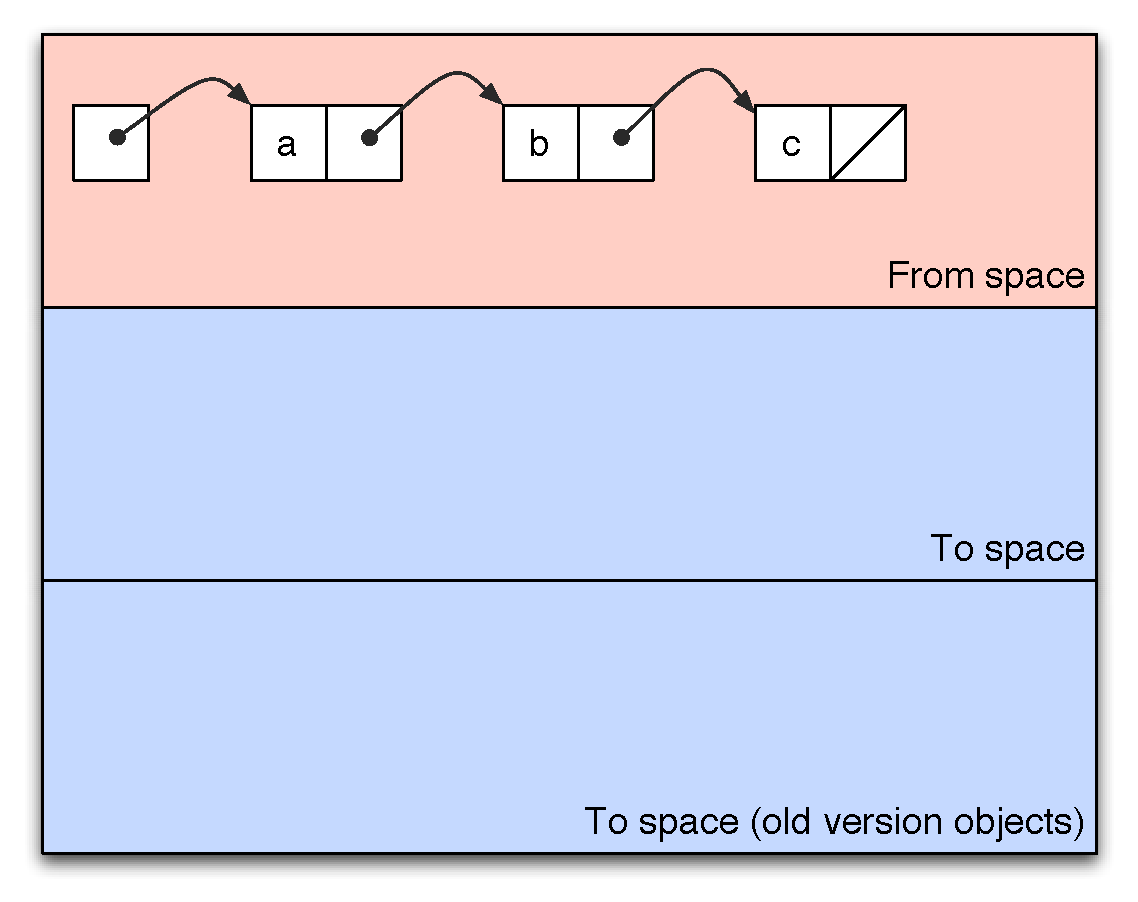
\includegraphics[scale=0.45]{images/singly-doubly/before-gc-copy}}%
\only<2>{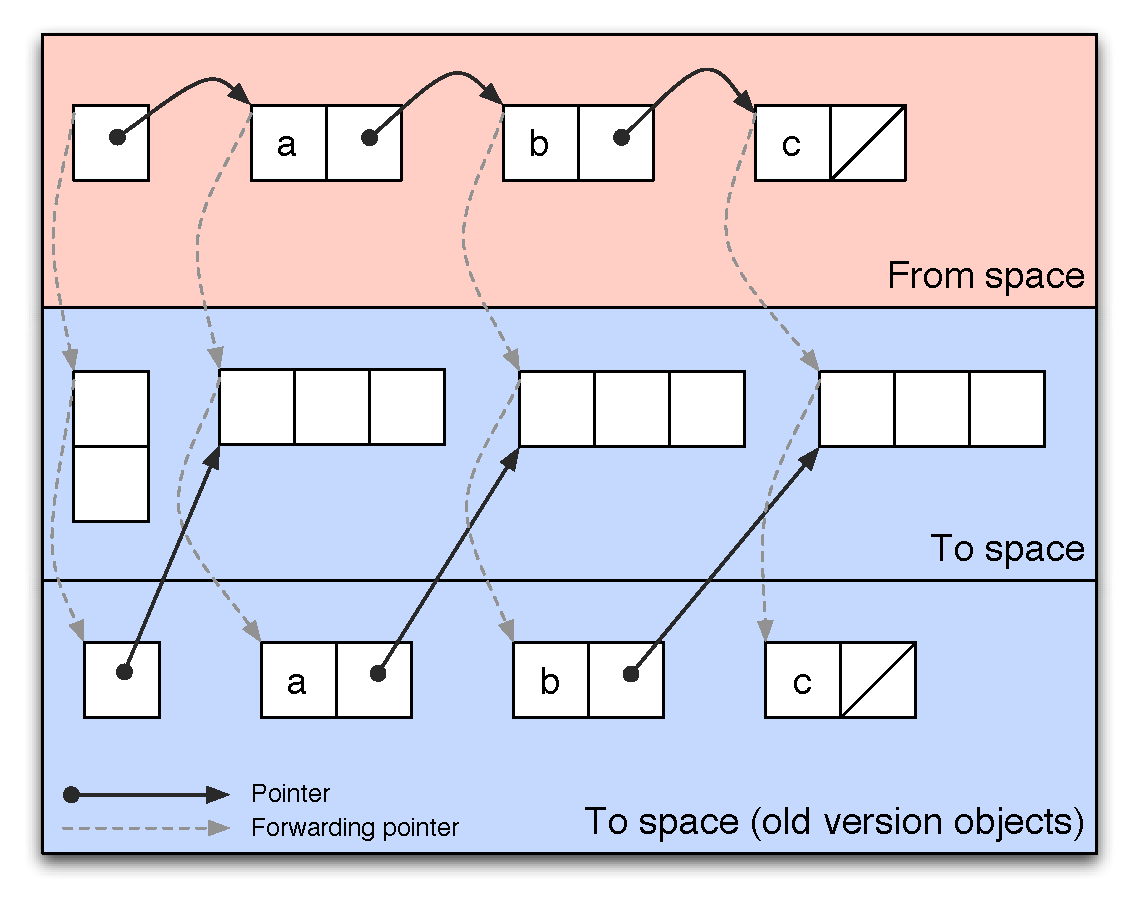
\includegraphics[scale=0.45]{images/singly-doubly/singly-doubly}}%
\only<3>{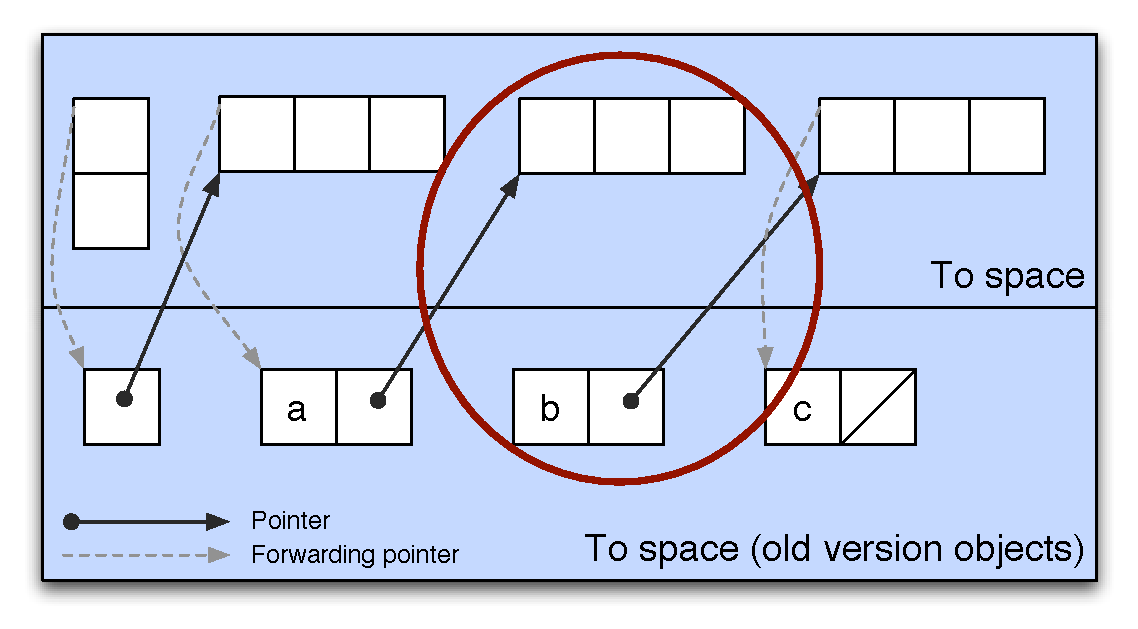
\includegraphics[scale=0.45]{images/singly-doubly/singly-doubly-transform-b-step-0}}
\only<4>{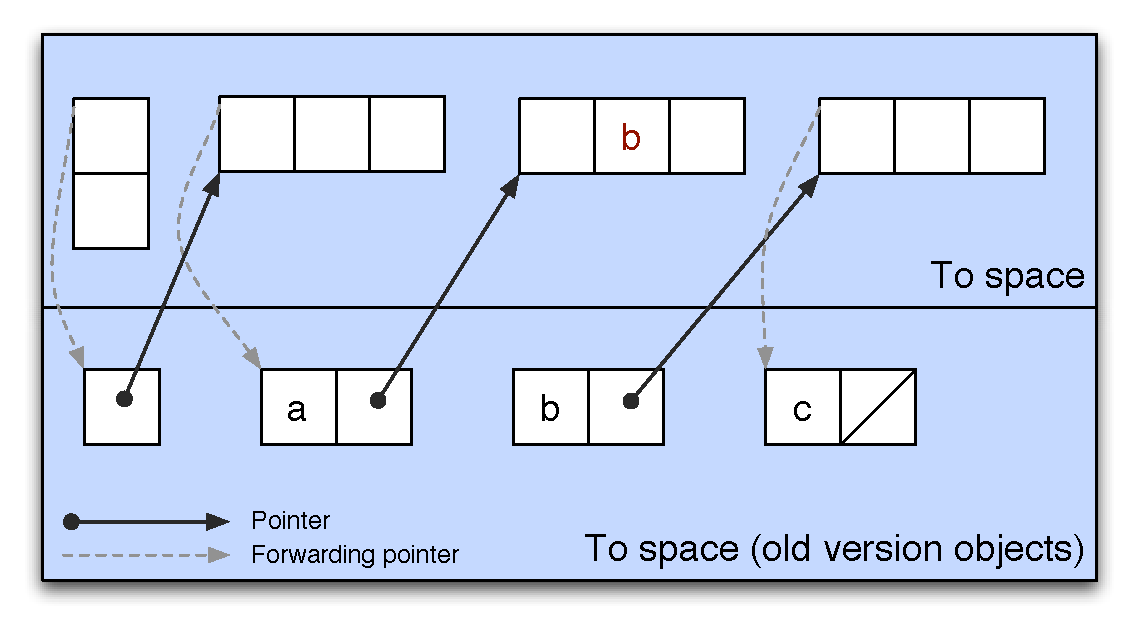
\includegraphics[scale=0.45]{images/singly-doubly/singly-doubly-transform-b-step-1}}
\only<5>{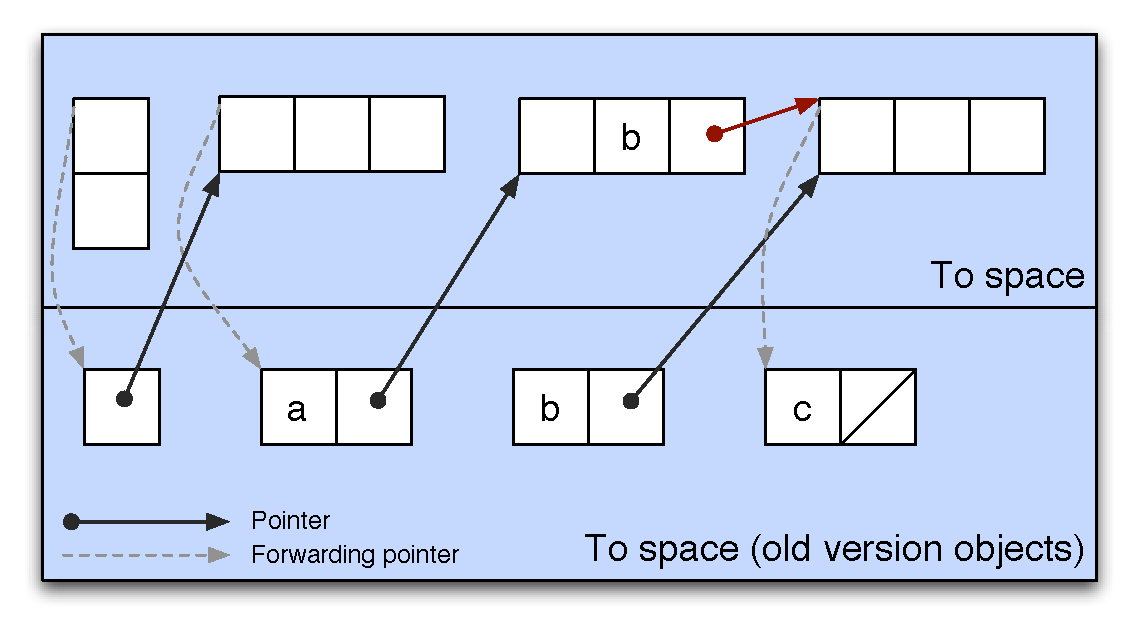
\includegraphics[scale=0.45]{images/singly-doubly/singly-doubly-transform-b-step-2}}
\only<6>{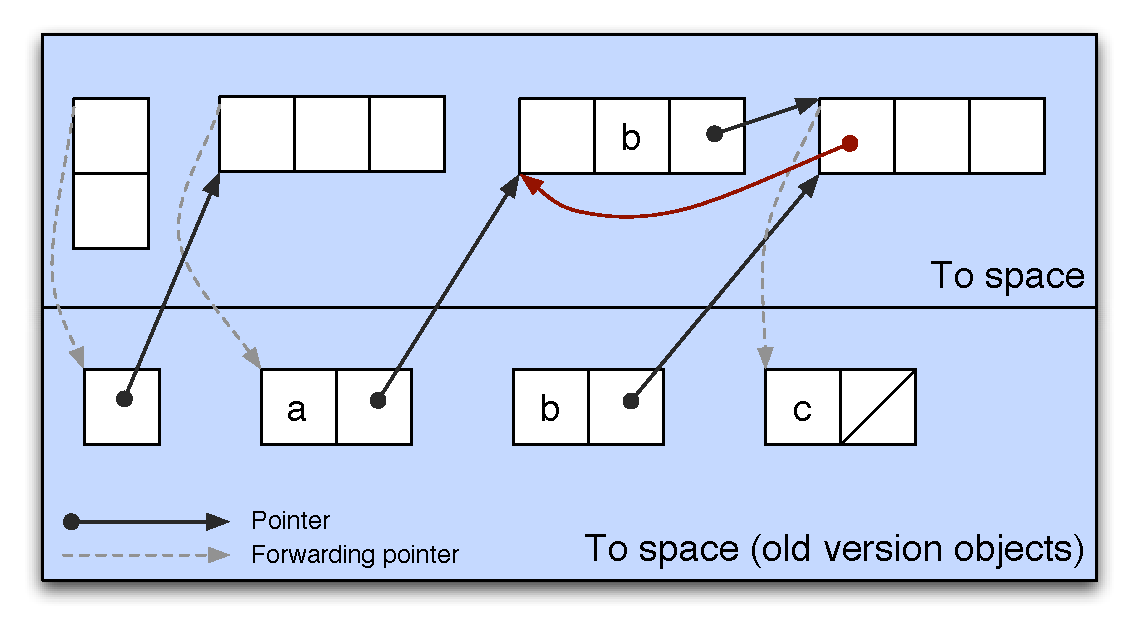
\includegraphics[scale=0.45]{images/singly-doubly/singly-doubly-transform-b-step-3}}
\only<7>{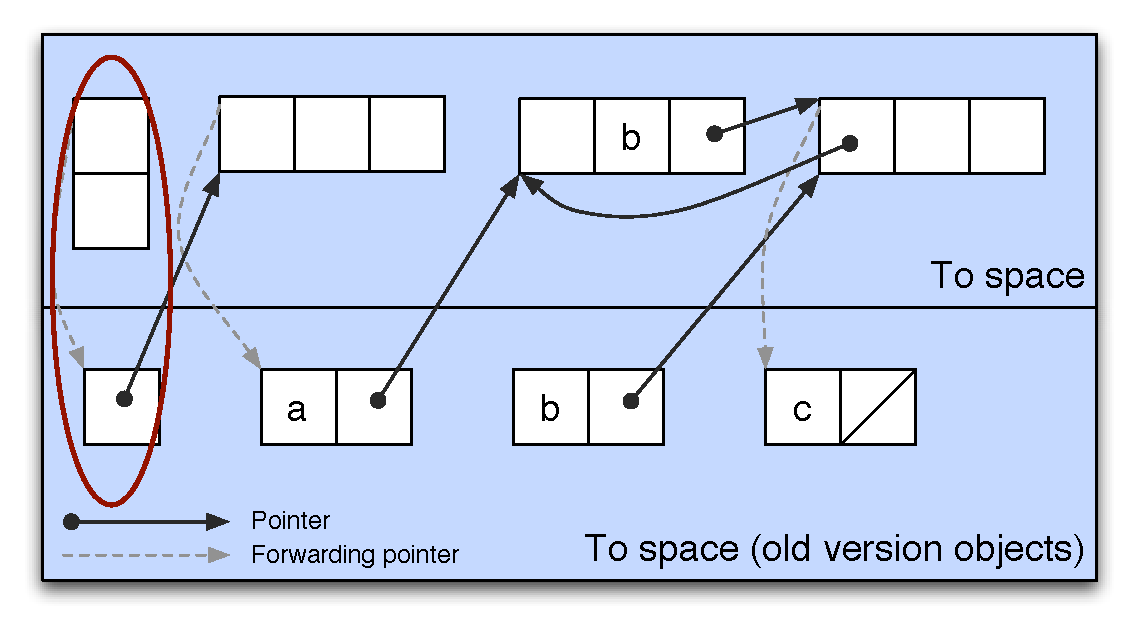
\includegraphics[scale=0.45]{images/singly-doubly/singly-doubly-transform-head-step-0}}
\only<8>{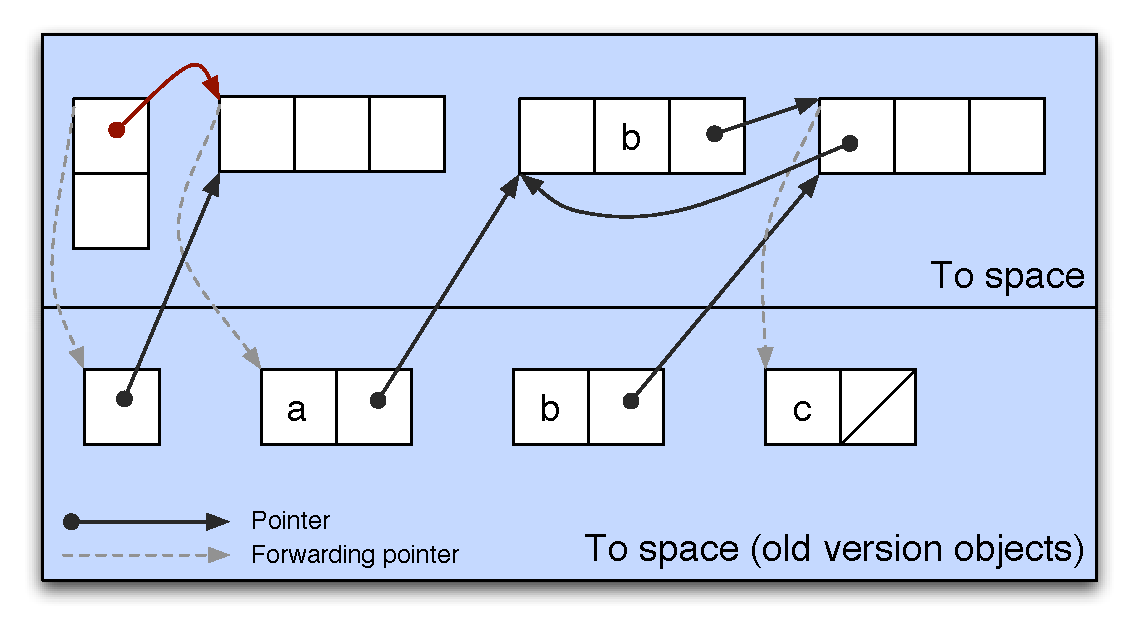
\includegraphics[scale=0.45]{images/singly-doubly/singly-doubly-transform-head-step-1}}
\only<9>{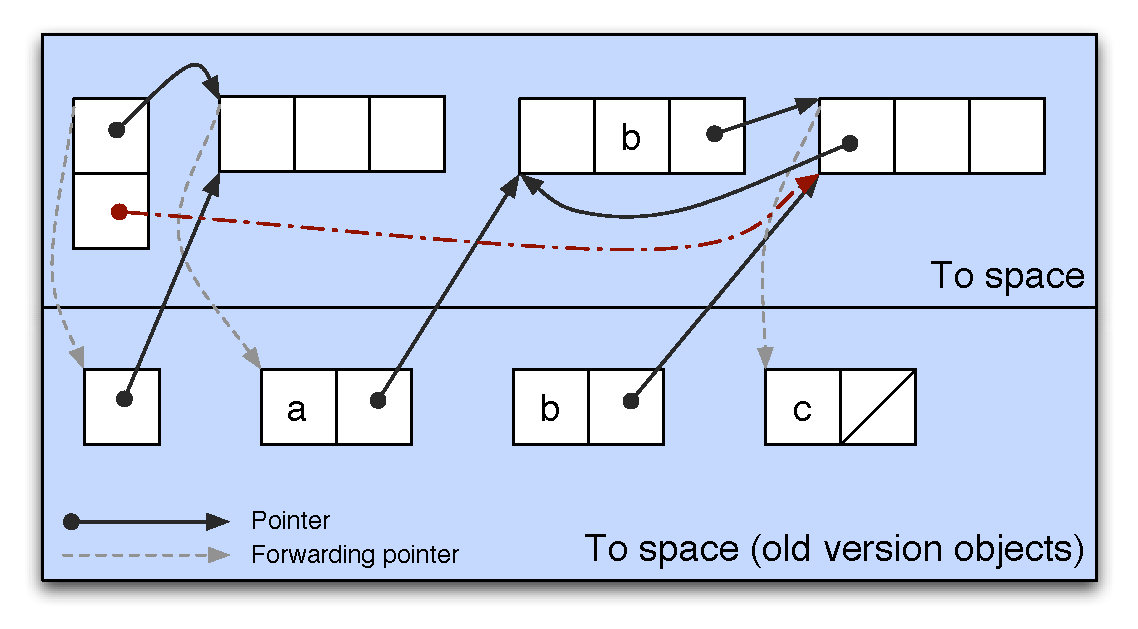
\includegraphics[scale=0.45]{images/singly-doubly/singly-doubly-transform-head-step-2}}
\only<10>{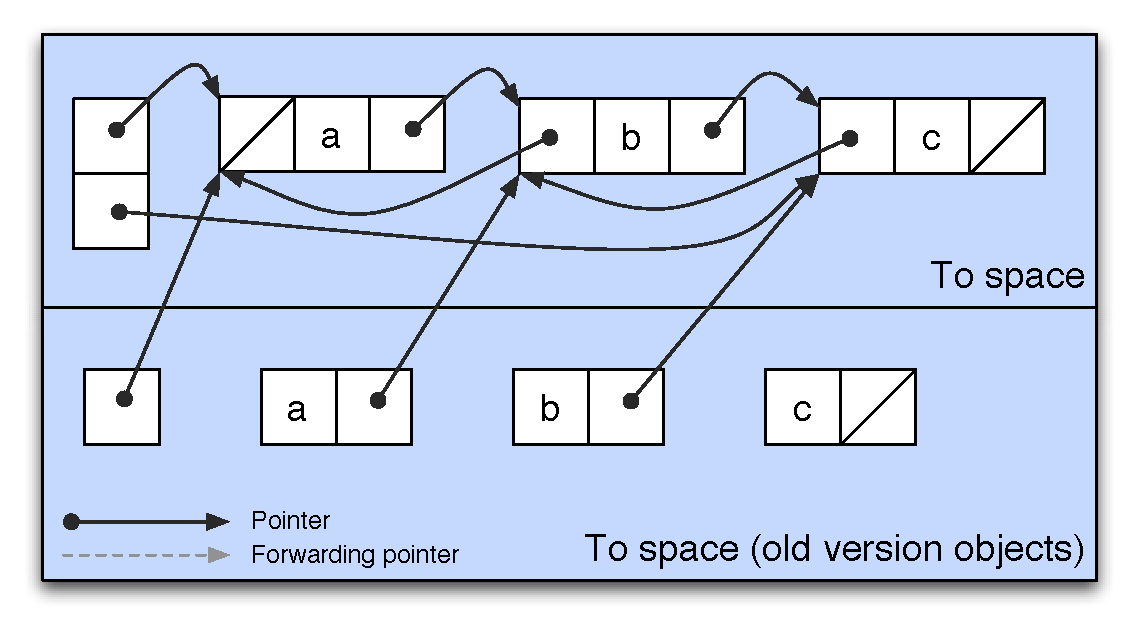
\includegraphics[scale=0.45]{images/singly-doubly/singly-doubly-transformed}}
\only<11>{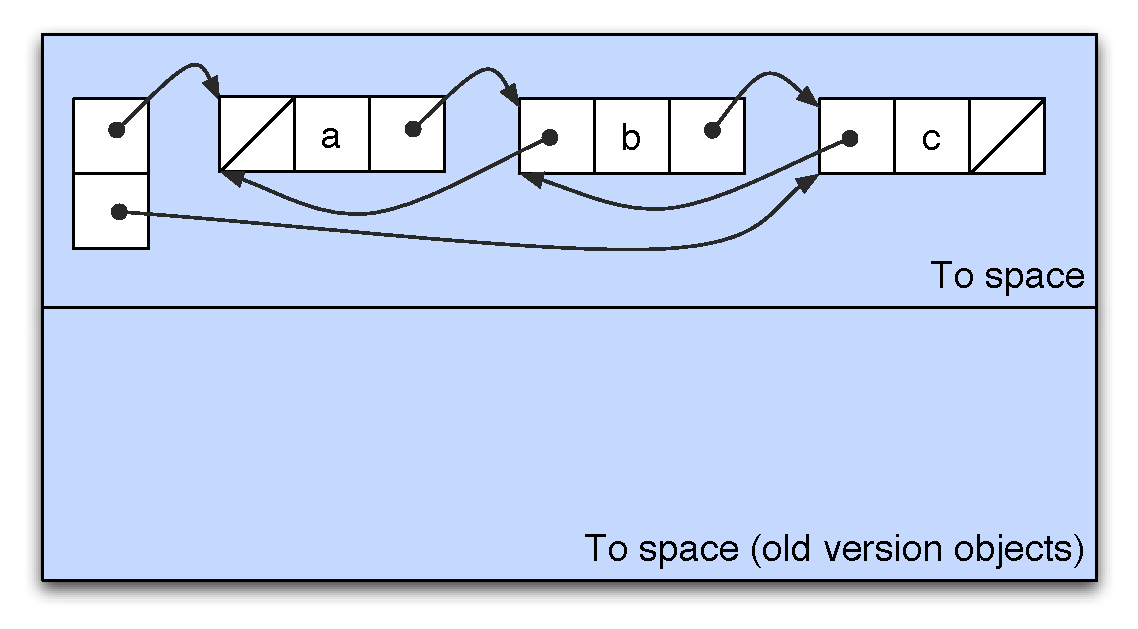
\includegraphics[scale=0.45]{images/singly-doubly/singly-doubly-transformed-final}}
\end{column}
\begin{column}{0.37\paperwidth}%
% Transform b, step 0
\only<3>{%
\begin{footnotesize}%
\noindent {\tt jvolveObject(Node to,}\\
{\tt\ \ \ \ old\_Node from) \{}\\
{\tt\ \ to.data = from.data;}\\
{\tt\ \ to.next = from.next;}\\
{\tt\ \ if (to.next != null)}\\
{\tt\ \ \ \ to.next.prev = to;}\\
{\tt \}}
\end{footnotesize}%
}%
% Transform b, step 1
\only<4>{%
\begin{footnotesize}%
\noindent {\tt jvolveObject(Node to,}\\
{\tt\ \ \ \ old\_Node from) \{}\\
{\tt\ \ \colorbox{yellow}{to.data = from.data;}}\\
{\tt\ \ to.next = from.next;}\\
{\tt\ \ if (to.next != null)}\\
{\tt\ \ \ \ to.next.prev = to;}\\
{\tt \}}
\end{footnotesize}%
}%
% Transform b, step 2
\only<5>{%
\begin{footnotesize}%
\noindent {\tt jvolveObject(Node to,}\\
{\tt\ \ \ \ old\_Node from) \{}\\
{\tt\ \ to.data = from.data;}\\
{\tt\ \ \colorbox{yellow}{to.next = from.next;}}\\
{\tt\ \ if (to.next != null)}\\
{\tt\ \ \ \ to.next.prev = to;}\\
{\tt \}}
\end{footnotesize}%
}%
% Transform b, step 3
\only<6>{%
\begin{footnotesize}%
\noindent {\tt jvolveObject(Node to,}\\
{\tt\ \ \ \ old\_Node from) \{}\\
{\tt\ \ to.data = from.data;}\\
{\tt\ \ to.next = from.next;}\\
{\tt\ \ \colorbox{yellow}{if (to.next != null)}}\\
{\tt\ \ \colorbox{yellow}{\ \ to.next.prev = to;}}\\
{\tt \}}
\end{footnotesize}%
}%
\end{column}
\end{columns}
\end{frame}


% \begin{frame}[t,fragile]{\DSU{} Garbage collector}%{A Sub-title is optional}
% \begin{itemize}
% \item Identical to Semispace for ``regular'' objects
% \item For objects to be transformed
%   \begin{itemize}
%   \item Copy the object to ToSpace (like Semispace)
%   \item Also, allocate an empty object in ToSpace for the new version
%   \end{itemize}
% \item Forwarding pointers point to the ``new version'' object
% \item No field can point to an ``old version'' object
% \end{itemize}
% \end{frame}

% \ifdraft{}{
% % 
%%%%%%%%%%%%%%%%%%%%%%%%%%%%%%%%%%%%%%%%%%%%%%%%%%%%%%%%%%%%%%%%%%%%%%%%
% Now, we show semispace with objects being updated.
%%%%%%%%%%%%%%%%%%%%%%%%%%%%%%%%%%%%%%%%%%%%%%%%%%%%%%%%%%%%%%%%%%%%%%%%
{
\begin{frame}[fragile]{\DSU{} garbage collector}%{A Sub-title is optional}
\setbeamercovered{invisible}
\begin{columns}[t]
\begin{column}[T]{0.67\paperwidth}
\begin{tikzpicture}
\begin{scope}
  % objects
  \uncover<1>{       \node[field] (root) at \objectRoot {root};                        }
  \uncover<2->{      \node[new space black field] (root) at \objectRoot {root};        }
                     \oldSpaceObject{A}{\objectA}
                     \oldSpaceObject{B}{\objectB}
                     \oldSpaceObject[dsu v0 object]{C}{\objectC}
                     \oldSpaceObject{D}{\objectD}
                     \oldSpaceObject{E}{\objectE}
                     \oldSpaceObject[dsu v0 object]{F}{\objectF}
                     \oldSpaceObject{G}{\objectG}
  % forwarding pointers
  \uncover<2->{      \forwardingPointer{A}                             }
  \uncover<3->{      \forwardingPointer{B}
                     \dsuForwardingPointer{C}                          }
  \uncover<4->{      \forwardingPointer{D}
                     \forwardingPointer{E}                             }
  \uncover<5->{      \dsuForwardingPointer{F}
                     \forwardingPointer{G}                             }
  % pointer arrows
  \uncover<1>   {    \path[regular]     (root.east)  to [out=330,in=120] (A.140)    ;          }
  \uncover<1>   {    \path[regular]     (A 0.center) to                (B.90)     ;            }
  \uncover<1>   {    \path[regular]     (A 1.center) to                (C.135)    ;            }
  \uncover<1-2> {    \path[regular]     (B 0.center) to                (D.135)    ;            }
  \uncover<1-2> {    \path[regular]     (B 1.center) to                (E.90)     ;            }
  \uncover<1-2> {    \path[regular]     (C 0.center) to                (F.135)    ;            }
  \uncover<1-2> {    \path[regular]     (C 1.center) to                (G.90)     ;            }
  \uncover<1-4> {    \path[regular]     (F 0.center) to                (A)        ;            }
                                                                      
  \uncover<2> {    \path[transparent]   (root.east)  to [out=0,in=120] (A.140)    ;            }
  \uncover<2> {    \path[transparent]   (A 0.center) to                (B.90)     ;            }
  \uncover<2> {    \path[transparent]   (A 1.center) to                (C.135)    ;            }
  \uncover<3> {    \path[transparent]   (B 0.center) to                (D.135)    ;            }
  \uncover<3> {    \path[transparent]   (B 1.center) to                (E.90)     ;            }
  \uncover<3> {    \path[transparent]   (C 0.center) to                (F.135)    ;            }
  \uncover<3> {    \path[transparent]   (C 1.center) to                (G.90)     ;            }
  \uncover<5> {    \path[transparent]   (F 0.center) to                (A)        ;            }

  \draw[draw,thin] (-4,-2.5) rectangle (4,0.5);
  \draw (4,0.5) node[anchor=north east,inner sep=1pt,font=\tiny] {FromSpace};

\end{scope}
\begin{scope}[yshift=-3.75cm]
  % objects
  \uncover<2>   {    \newSpaceGreyObject{A'}{\objectAprime}                          }
  \uncover<3->  {    \newSpaceBlackObject{A'}{\objectAprime}                         }

  \uncover<3>   {    \newSpaceGreyObject{B'}{\objectBprime}                          }
  \uncover<4->  {    \newSpaceBlackObject{B'}{\objectBprime}                         }

  \uncover<3-4> {    \dsuNewSpaceGreyObject{C'}{\objectCprime}                       }
  \uncover<5-10>{    \dsuNewSpaceBlackObject{C'}{\objectCprime}                      }
  \uncover<3->  {    \newSpaceVersionOneEmptyObject{C'}{\objectCprimeVersionOne}     }

  \uncover<4-5> {    \newSpaceGreyObject{D'}{\objectDprime}                          }
  \uncover<6->  {    \newSpaceBlackObject{D'}{\objectDprime}                         }

  \uncover<4-6> {    \newSpaceGreyObject{E'}{\objectEprime}                          }
  \uncover<7->  {    \newSpaceBlackObject{E'}{\objectEprime}                         }

  \uncover<5-7> {    \dsuNewSpaceGreyObject{F'}{\objectFprime}                       }
  \uncover<8-10>{    \dsuNewSpaceBlackObject{F'}{\objectFprime}                      }
  \uncover<5->  {    \newSpaceVersionOneEmptyObject{F'}{\objectFprimeVersionOne}     }

  \uncover<5-8> {    \newSpaceGreyObject{G'}{\objectGprime}                          }
  \uncover<9->  {    \newSpaceBlackObject{G'}{\objectGprime}                         }

  % pointer arrows
  \uncover<2->  {    \path[regular] (root.west)   to [out=220,in=95] (A'.north west);    }
  \uncover<2>   {    \path[regular] (A' 0.center) to [out=130,in=180] (B.west);
                     \path[regular] (A' 1.center) to [out=70,in=180]  (C.west);           }
  \uncover<3->  {    \path[regular] (A' 0.center) to [out=80,in=135]  (B'.150);          
                     \path[regular] (A' 1.center) to [out=270,in=110] (C' v1.north west); }
                                                                                         
  \uncover<3>   {    \path[regular] (B' 0.center) to                  (D.south);         
                     \path[regular] (B' 1.center) to                  (E.south);          }
  \uncover<4->  {    \path[regular] (B' 0.center) to [out=300,in=240] (D'.215);          
                     \path[regular] (B' 1.center) to [out=330,in=240] (E'.215);           }
                                                                                         
  \uncover<3-4> {    \path[regular] (C' 0.center) to                  (F.south);         
                     \path[regular] (C' 1.center) to                  (G.south west);     }
  \uncover<5-10>{    \path[regular] (C' 0.center) to [out=255,in=105]  (F' v1.north west);          
                     \path[regular] (C' 1.center) to [out=70,in=150]  (G'.150);           }
                                                                                         
  \uncover<5-7> {    \path[regular] (F' 0.center) to [out=30,in=325]  (A);                }
  \uncover<8-10>{    \path[regular] (F' 0.center) to [out=215,in=330] (A'.215);           }

  % transparent arrows
  \uncover<3>   {    \path[transparent] (A' 0.center) to [out=130,in=180] (B.west);
                     \path[transparent] (A' 1.center) to [out=70,in=180]  (C.west);       }

  \uncover<4>   {    \path[transparent] (B' 0.center) to                  (D.south);
                     \path[transparent] (B' 1.center) to                  (E.south);      }

  \uncover<5>   {    \path[transparent] (C' 0.center) to                  (F.south);
                     \path[transparent] (C' 1.center) to                  (G.south west); }

  \uncover<8>   {    \path[transparent] (F' 0.center) to [out=30,in=325]  (A);            }

  % v1 arrows
  \uncover<10-> {    \path[regular] (C' v1 0.center) to [out=30,in=120]   (F' v1.north west);
                     \path[regular] (C' v1 1.center) to                   (G'.210);          
                     \path[regular] (F' v1 0.center) to [out=180,in=315]  (A'.215);
                }
  

  \draw[draw,thin] (-4,-2) rectangle (4,0.5);
  \draw (4,-2) node[anchor=south east,inner sep=1pt,font=\tiny] {ToSpace};
\end{scope}
\end{tikzpicture}
\end{column}
\begin{column}[T]{0.25\paperwidth}
\begin{block}{}
\begin{tikzpicture}
\tikzstyle{column 2}=[anchor=west]
\matrix [row sep=0.5ex] {
\node[dsu v0 field] {};          & \node {\tiny To be transformed}; \\
\node[dsu v1 empty field] {};    & \node {\tiny $v_1$ object}; \\
};
\end{tikzpicture}
\end{block}

\begin{block}{}
\begin{footnotesize}
\only<1>{
The same heap as before. Objects to be transformed are highlighted.
}
\only<2>{
Copy A.
}
\only<3>{
Scan A'. Copy B and C. In addition an empty object C'$v_1$ is allocated.
\alert{A' points to this copy and not the old one.}
}
\only<4>{
Scan B'.
}
\only<5>{
Scan C'.
}
\only<6>{
Scan D'.
}
\only<7>{
Scan E'.
}
\only<8>{
Scan F'.
}
\only<9>{
GC is now complete. No field can point to C'$v_0$ or F'$v_0$. Pointers to C and
F point to $v_1$ (empty) objects. \texttt{memcpy(v\_1, v\_0);} will give us a valid
heap.}
\only<10>{
Setting fields of C'$v_1$ and F'$v_1$.
}
\only<11>{
C'$v_0$ and F'$v_0$ can be reclaimed.
}
\end{footnotesize}
\end{block}
\end{column}
\end{columns}
\end{frame}
}

% vim:tw=0:nospell

% {
\begin{frame}[fragile]{\DSU{} Garbage collector}%{A Sub-title is optional}
\setbeamercovered{invisible}
\begin{center}
\begin{tikzpicture}
  % objects
                  \node[field] (root) at \objectRoot {root};
                  \oldSpaceObject{A}{\objectA}
                  \oldSpaceObject{B}{\objectB}
\uncover<-2>{     \dsuOldSpaceVersionZeroObject{C}{\objectC}                  }
                  \oldSpaceObject{D}{\objectD}
                  \oldSpaceObject{E}{\objectE}
\uncover<-2>{     \dsuOldSpaceVersionZeroObject{F}{\objectF}                  }
                  \oldSpaceObject{G}{\objectG}

                  \dsuOldSpaceVersionOneObject{C}{\objectCVersionOne}
                  \dsuOldSpaceVersionOneObject{F}{\objectFVersionOne}

                  % pointer arrows
                  \path[regular]     (root.east)  to [out=330,in=120]     (A.140);
                  \path[regular]     (A 0.center) to                      (B.90);
                  \path[regular]     (A 1.center) to                      (C v1.190);
                  \path[regular]     (B 0.center) to                      (D.135);
                  \path[regular]     (B 1.center) to                      (E.90);
\uncover<-2>{     \path[regular]     (C 0.center) to [out=180,in=90]      (F v1.north west);
                  \path[regular]     (C 1.center) to                      (G.90);
                  \path[regular]     (F 0.center) to                      (A);                       }

\uncover<2-3>{    \path[regular]     (C v1 0.center) to [out=180,in=120]  (F v1.north west);
                  \path[regular]     (C v1 1.center) to                   (G.60);
                  \path[regular]     (F v1 0.center) to                   (A);                       }

  \draw[draw,thin] (-4,-3.5) rectangle (4,0.5);
\end{tikzpicture}
% \begin{block}{}
% Loren ipsum. Hello World. Hello World. Hello World.  Loren ipsum. Hello World.
% Hello World. Hello World.  Loren ipsum. Hello World. Hello World. Hello World.
% Loren ipsum. Hello World.\footnote{This is a footnote} Hello World. Hello World.  Loren ipsum. Hello World.
% Hello World. Hello World.
% \end{block}
\end{center}
\end{frame}
}

% vim:tw=0:nospell

% % {
\begin{frame}[fragile]{Revisiting transformation functions}%{A Sub-title is optional}
\setbeamercovered{invisible}
\begin{center}
\begin{tikzpicture}
  % objects
  \node[field] (root) at \objectRoot {root};
  \oldSpaceObject{A}{\objectA}
  \oldSpaceObject{B}{\objectB}
  \dsuOldSpaceVersionZeroObject{C}{\objectC}
  \oldSpaceObject{D}{\objectD}
  \oldSpaceObject{E}{\objectE}
  \dsuOldSpaceVersionZeroObject{F}{\objectF}
  \oldSpaceObject{G}{\objectG}
  \dsuOldSpaceVersionOneObject{C}{\objectCVersionOne}
  \dsuOldSpaceVersionOneObject{F}{\objectFVersionOne}

  % pointer arrows
  \path[regular]     (root.east)  to [out=330,in=120]     (A.140);
  \path[regular]     (A 0.center) to                      (B.90);
  \path[regular]     (A 1.center) to                      (C v1.190);
  \path[regular]     (B 0.center) to                      (D.135);
  \path[regular]     (B 1.center) to                      (E.90);
  \path[regular]     (C 0.center) to [out=180,in=90]      (F v1.north west);
  \path[regular]     (C 1.center) to                      (G.90);
  \path[regular]     (F 0.center) to                      (A);

  \draw[draw,thin] (-4,-3.5) rectangle (4,0.5);
\end{tikzpicture}
\begin{block}{We have an ordering problem}
\texttt{(C $v_0$).field0.field0} might be uninitialized
\end{block}
\end{center}
\end{frame}
}

% vim:tw=0:nospell

% }

% \begin{frame}[t,fragile]{Revisiting transformation functions}%{A Sub-title is optional}
% Solutions to the ordering problem \\
% \begin{itemize}
% \item Programmer can invoke a VM function that will transform objects on
% demand. Moves burden of safety to the programmer
% \uncover<2>{
% \item Insert read barrier code to perform this check when compiling the
% transformation function
% \item Perform some static analysis to determine an order to queue
% objects
% }
% \end{itemize}
% \end{frame}

\section{Experience}
\label{sec:experience}

To evaluate \DSU, we used it to update three open-source servers written
in Java: the Jetty webserver\footnote{\url{http://www.mortbay.org}},
JavaEmailServer,\footnote{\url{http://www.ericdaugherty.com/java/mailserver/}}
an SMTP and POP e-mail server, and CrossFTP server.\footnote{\url{http://www.crossftp.com/}}
These programs belong to a class that
should benefit from DSU because they typically run continuously. DSU
would enable deployments to incorporate bug fixes or add new features
without having to halt currently-running sessions.  

We explored
updates corresponding to releases made over roughly one to two years
of each program's lifetime.  Of the 22 updates we considered, \DSU{} could
support 20 of them---the two updates we could not apply changed
classes with infinitely-running methods, and thus no safe point could
be reached.  To our knowledge, no existing DSU system
for Java could support all these updates; indeed, previous systems
with simple support for updating method bodies would be able to handle only 9 of the 22 updates.  Although \DSU{} cannot support every
update, it is the first DSU system for Java
that has been shown to support changes to realistic programs as they
occur in practice over a long period of time.

In the rest of this section, we first examine the performance impact of
\DSU{}, and then look at updates to each of the three applications in
detail.

\begin{figure}[t]
\begin{small}
\begin{center}
\begin{tabular}{|l|c|c|c|c|} \hline \T
Config.                & \multicolumn{2}{c|}{Throughput (MB/s)}  & \multicolumn{2}{c|}{Latency (ms)} \\ \cline{2-5}
                       & Median   & Quartiles \T                 & Median & Quartiles                \\ \hline \T
\JikesRVM{}            & 122.437  & 121.44--123.32               & 0.442  & 0.394--0.496             \\
\DSU{}                 & 121.308  & 121.12--121.41               & 0.349  & 0.341--0.351             \\
\DSU{} upd             & 121.242  & 121.09--121.29               & 0.345  & 0.341--0.349             \\ \hline
\end{tabular}
\end{center}
\end{small}
% \caption{Throughput and latency measurements for Jetty webserver v5.1.6
% showing median and semi-interquartile range\label{tab:jetty}}
\begin{center}
\scalebox{0.63}{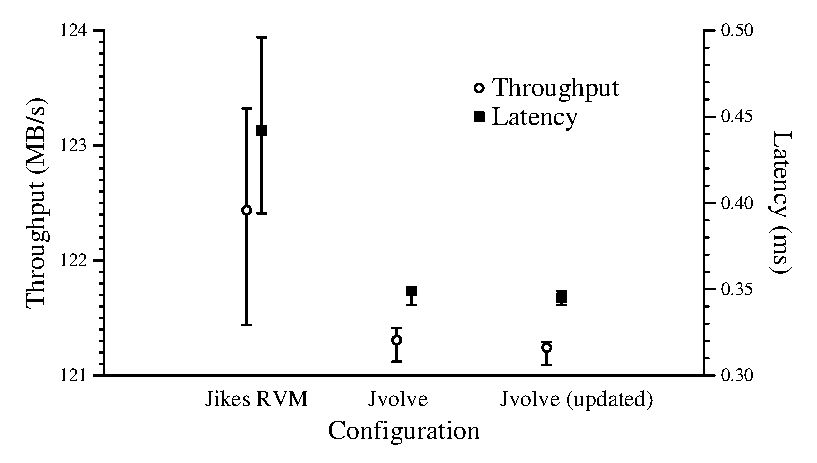
\includegraphics{graphs/jetty-throughput-latency}}
\caption{Throughput and latency measurements of Jetty webserver v5.1.6\label{fig:jetty}}
\end{center}
\end{figure}

\begin{table*}[t]
\begin{footnotesize}
\begin{center}
\begin{tabular}{|r|r|rrrrrrrrrrr|}
                                                                                                                                   \hline
\multirow{2}{*}{\# objects}     & \multicolumn{1}{c}{Heap}   & \multicolumn{11}{|c|}{Fraction of updated objects \T}            \\
                                & \multicolumn{1}{c|}{size}  &
                       0\%  &   10\%  &   20\%  &   30\%  &   40\%  &   50\%  &   60\%  &   70\%  &   80\%  &   90\%  &  100\%  \\ \hline
\multicolumn{13}{|c|}{Garbage collection time (ms) \T}                                                                          \\ \hline \T
 280000 &  160 MB &    78.2 &    81.3 &    83.1 &    89.3 &    99.0 &   103.2 &   108.3 &   113.2 &   113.3 &   120.3 &   120.0 \\
 770000 &  320 MB &   148.9 &   165.0 &   181.9 &   195.8 &   213.2 &   223.2 &   237.0 &   249.0 &   262.0 &   269.5 &   278.6 \\
1760000 &  640 MB &   313.3 &   347.7 &   382.9 &   416.0 &   449.8 &   478.9 &   506.8 &   534.0 &   558.8 &   583.7 &   601.5 \\
3670000 & 1280 MB &   615.4 &   694.6 &   763.0 &   833.6 &   900.1 &   965.9 &  1019.0 &  1076.4 &  1129.9 &  1181.2 &  1217.5 \\ \hline
\multicolumn{13}{|c|}{Running transformation functions (ms) \T}                                                                 \\ \hline \T
 280000 &  160 MB &     0.1 &    13.0 &    23.2 &    34.6 &    43.9 &    54.0 &    62.7 &    74.5 &    84.1 &    93.9 &   104.2 \\
 770000 &  320 MB &     0.1 &    33.7 &    63.1 &    91.2 &   116.8 &   145.4 &   173.9 &   201.0 &   231.3 &   262.0 &   292.6 \\
1760000 &  640 MB &     0.1 &    77.9 &   143.9 &   207.7 &   269.5 &   333.7 &   397.6 &   464.0 &   534.6 &   604.5 &   674.9 \\
3670000 & 1280 MB &     0.1 &   160.8 &   299.2 &   429.4 &   560.2 &   693.8 &   827.3 &   975.0 &  1119.6 &  1263.7 &  1405.4 \\ \hline
\multicolumn{13}{|c|}{Total DSU pause time (ms) \T}                                                                             \\ \hline \T
 280000 &  160 MB &    82.8 &    99.0 &   109.5 &   128.0 &   147.6 &   161.2 &   174.5 &   192.8 &   202.5 &   218.8 &   228.1 \\
 770000 &  320 MB &   153.6 &   202.9 &   249.0 &   291.4 &   334.5 &   372.6 &   414.8 &   455.4 &   498.1 &   535.3 &   576.8 \\
1760000 &  640 MB &   316.6 &   429.5 &   530.5 &   627.2 &   723.4 &   816.0 &   908.6 &  1002.6 &  1097.5 &  1191.5 &  1281.2 \\
3670000 & 1280 MB &   618.7 &   859.0 &  1065.9 &  1269.9 &  1466.1 &  1663.6 &  1850.8 &  2054.2 &  2253.1 &  2448.5 &  2627.9 \\ \hline
\end{tabular}
\end{center}
\end{footnotesize}
\caption{Microbenchmark results: \DSU{} update pause time (in ms) for various heap sizes}
\label{tab:microbench}
\end{table*}


\subsection{Performance}
\label{subsec:performance}

The main performance impact of \DSU{} is the cost of applying an update;
once updated, the application eventually runs without further overhead.  To confirm
%MWH: added "eventually" here because of the cost of recompilation.
%We don't actually measure this though.  Is that a problem?
this claim, we measured the throughput and latency of two Jetty versions while running on
stock \JikesRVM{} and on \DSU{} after dynamically updating to the next version. The performance of these configurations is
essentially identical.

% We report
% on this experiment in Section~\ref{subsec:jetty-perf}.

The cost of applying an update is the time to load any new classes, invoke a
full heap garbage collection, and to apply the transformation methods on
objects belonging to updated classes.
Roughly,
the time to suspend threads and check
that the application is in a safe-point is less than a millisecond, and classloading
time is usually less than 20ms.
% (Classloading could occur in parallel with normal execution.) 
Therefore the update disruption time is primarily
due to the GC and object transformers, and is proportional
to the size of the heap and the fraction of objects being transformed.  We
wrote a simple microbenchmark to measure these overheads.
% Section~\ref{subsec:microbench}
This experiment shows that object
transformation is the dominant cost.

We conducted all our experiments on an Intel Core 2 Quad machine running at 2.4 GHz machine with 2 GB of RAM.
The machine ran Ubuntu 7.10 on Linux kernel version 2.6.22. We implemented
\DSU{} on top of \JRVMVersion{}.

% We also have microbenchmarks where we compare the
% overhead added as a result of running the transformer function.

% \input{experience/performance-jetty-table}
% \input{experience/performance-jetty-graph}
% \input{experience/performance-microbench-table}

\paragraph{Jetty performance.}
To see the effect of updating on application performance, we measured Jetty
under various configurations using httperf, a webserver
benchmarking tool.\footnote{\url{http://www.hpl.hp.com/research/linux/httperf}}  We used httperf to issue roughly 800 new connection
requests/second, which we observed to be Jetty's saturation rate.
Each connection makes 5 serial requests for a 40 Kbyte file. Httperf
reports average throughput and average per-request latency over a 60 second period. We
ran this experiment 21 times and report the median and
quartiles of the throughput and latency reports. With 21 runs, the range between
the quartiles serves as a 98\% confidence interval~\cite{PrattGibbons81}.
In order to eliminate network traffic
effects, we ran the server on two cores of a quad-core machine and the
client on another core.

Figure~\ref{fig:jetty} shows our results in tabular form and plotted graphically.  The second and third columns
of the table
report the median throughput and the range between the two quartiles.
The third column and fourth column report the median latency and the
inter-quartile range.  The
first and seconds rows illustrate the performance of Jetty version 5.1.6
running on stock \JikesRVM{} and \DSU, respectively. The third row shows
the performance on \DSU{} of Jetty 5.1.6 dynamically updated from version
5.1.5 prior to the start of the experiment.
% \todo{Find a way to introduce the graph} Figure~\ref{fig:jetty} plots the results shown in the table.
The performance of the two \DSU{} configurations
is essentially identical: the two configurations' corresponding
inter-quartile ranges largely overlap.
The performance of \DSU{} is also quite similar to the performance of
stock \JikesRVM.  There are many small differences between \DSU{} and the stock
implementation that change VM code size, code layout, and garbage
collection behavior.  These differences may impact performance
directly and they may indirectly affect other elements of the VM,
such as the timing of garbage collections and JIT
optimizations (such indirect effects make VMs notoriously difficult to
benchmark~\cite{dacapo-cacm}).


%%% Local Variables: 
%%% mode: latex
%%% TeX-master: "../pldi64"
%%% End: 

% \input{experience/performance-microbench-table}
\input{experience/performance-microbench-graph}

\paragraph{Microbenchmarks.}
The two dominant factors that determine \DSU{} update time are the time to
perform a GC, determined by the number of objects, and the time to run
object transformers, determined by the fraction of objects being
updated.  To measure the cost of each, we devised a simple 
microbenchmark that creates an array of objects and transforms a specified
fraction of these objects when a \DSU{} update is triggered. The
microbenchmark has two simple classes, \texttt{Change} and
\texttt{NoChange}. Both contain three integer fields, and three reference
fields that are always {\tt null}. The update adds an integer field to
{\tt Change}. The user-provided object transformation function copies the
existing fields and initializes the new field to zero.
% The benchmark contains two arrays,
% one for \texttt{Change} objects and one for \texttt{NoChange} objects.
We measure the cost of performing an update while varying the total
number of objects and the fraction of objects of each type. The number of
objects is the maximum that can fit in heap sizes 32, 64, 128 and 256
MB.  Note that \JikesRVM{}'s heap includes VM data structures as well. We
measure the running time in a generous heap, five times the minimum required size, such that the only collections are those DSU triggers. We report the
median of 21 runs.

Table~\ref{tab:microbench} shows the elapsed time
while varying the number of total objects and the fraction of the objects that are updated.  The
variance was insignificant, so we do not report it.   % KSM: I deleted the first row, since it is the only one with this problem, which is due to other costs dominating, e.g., stack walking etc. because apparently copying 40,000 objects takes no time at all. \todo{some of the
%   results are unintuitive; e.g., the time goes down as you move to the
%   right, sometimes.  Make a comment here about that being the way of
%   things with sophisticated machines?  Can't blame it on the
%   variance.}
The first group of rows reports
garbage collection time, the second group reports the time to transform
all updated objects, and the final group reports the total update time, which
includes the sum of the GC and transformation time, the time to load and install the updated classes, synchronize
running threads, and find a DSU safe point. 
The first column of the table shows the number of objects in the test, and
the second column the heap size. Columns 3 though 13 show pause times for
varying fractions (from 0\% to 100\%) of updated objects. 
% Looking at
% the last column of the table, we can see that the GC time results
% (first group of rows) for
% various heap sizes are roughly the same as the transformation time
% results (second group of rows), showing the time to transform an
% object to be roughly equal to the time to copy an object in the collector.

To shed light on the results in the table,
Figure~\ref{fig:microbench} plots collection time, transformer time and
total update time for the microbenchmark with 3.67 million objects in a
1280 MB heap.  The figure shows that the costs of garbage collection and
transformation increase  as a function of the number of changed objects.  The slope of the ``GC time'' line illustrates the cost to deal
with an increasing number of transformed objects.  This cost includes
creating an additional copy of each transformed object; creating the
update log entry with a pointer to the old and new copy; and caching a
pointer to the old copy from the new copy.  The slope of the
``Running transformers'' line illustrates the added cost of iterating
over the update log and actually running the transformers.  This extra
processing to handle transforming objects increases the total pause
time with all objects updated by roughly four times compared to the
pause time with no object updated.  The ``Running
Transformers'' line is steeper than the ``GC time'' line, revealing that
the cost of running transformers is higher than the extra copying cost
incurred during GC\@.

Transformations are more expensive than standard copying GC. The GC uses
\texttt{memcopy}, which is highly optimized, whereas our transformer
functions use reflection to look up \texttt{jvolveObject}, and this
function copies one field at a time.  One optimization would be to eliminate the log by copying
the old and new objects to their own space and % appending to each one a
% pointer to their corresponding new object.
walking through and transforming each object.
The cost of reflection could be
reduced by caching the lookup, but even then a na\"ively compiled
field-by-field copy is much slower than the collector's
highly-optimized copying loop.  % Another possible optimization is to
% specially compile transformers to replace idiomatic use of copying
% assignments to contiguous fields by a \texttt{memcopy} over the
% corresponding range.


%%% Local Variables: 
%%% mode: latex
%%% TeX-master: "../pldi64"
%%% End: 



\newcommand{\ChangedClassesColumn}{third}
\begin{table}
\begin{footnotesize}
\begin{center}
\begin{tabular}{|l||c||c|c|c|r|c|c|} \hline \T
Ver.    & \#      & \multicolumn{6}{c|}{\# changed} \\
        & classes & \multicolumn{1}{c|}{classes} & \multicolumn{3}{c|}{methods} & \multicolumn{2}{c|}{fields} \\
        & added   &         & add & del & \multicolumn{1}{c|}{chg}             & add & del \\ \hline \hline \T
5.1.1   & 0       & 14      &\ 4  & 1   &  38/0            &  0  & 0   \\
5.1.2   & 1       &\ 5      &\ 0  & 0   &  12/1            &  0  & 0   \\
5.1.3*  & 3       & 15      & 19  & 2   &  59/0            & 10  & 1   \\
5.1.4   & 0       &\ 6      &\ 0  & 4   &   9/6            &  0  & 2   \\
5.1.5   & 0       & 54      & 21  & 4   & 112/8            &  5  & 0   \\
5.1.6   & 0       &\ 4      &\ 0  & 0   &  20/0            &  5  & 6   \\
5.1.7   & 0       &\ 7      &\ 8  & 0   &  11/2            &  9  & 3   \\
5.1.8   & 0       &\ 1      &\ 0  & 0   &   1/0            &  0  & 0   \\
5.1.9   & 0       &\ 1      &\ 0  & 0   &   1/0            &  0  & 0   \\
5.1.10  & 0       &\ 4      &\ 0  & 0   &   4/0            &  0  & 0   \\ \hline
\end{tabular}
\end{center}
\end{footnotesize}
\caption{Summary of updates to Jetty}
\label{tab:jetty-changes}
\end{table}

\subsection{Jetty webserver}
\label{subsec:jetty}

Jetty is a popular webserver written in Java. It supports static
and dynamic content and can be embedded 
within other Java applications. \JikesRVM, and thus \DSU, is not able to run the
most recent versions of Jetty (6.x).  Therefore we considered 11
versions, consisting of 5.1.0 through 5.1.10 (the last version prior to
version 6).  Version 5.1.10 contains 317 classes and about 45,000 lines
of code.  Table~\ref{tab:jetty-changes} shows a summary of the changes
in each update.  Each row tabulates the changes relative
to the prior version. For the column listing changed methods, the
notation $x/y$ indicates that $x+y$ methods were changed, where $x$
changed in body only, and $y$ changed their type signature as well.
For dynamic updating systems that only support changes to method
bodies, only the first and last three of the ten updates could be
supported, since the rest either change method signatures
and/or add or delete fields.

\paragraph{Reaching a safe point in Jetty.}
We  successfully wrote dynamic updates to all
versions of Jetty that we examined. For each version starting at 5.1.0, we ran
Jetty under full load. After 30 seconds we tried to apply the update to the
next version. We did this five times per version.  Other than the
update to 5.1.3, all versions immediately 
reached a safe point every time, with no need of return barriers.

We could not apply the update to version 5.1.3 (denoted with an
asterisk in the table) 
because \DSU{} was never able to reach a safe point. The update modified
{\tt ThreadedServer.accept\-Socket()}, a method that waits for a connection
from the client, and this method is nearly always on stack. 
We installed a return barrier that is triggered when {\tt
  acceptSocket} returns, but this barrier is not sufficient to perform the
update since the main methods of several threads were themselves
modified. For example, we also install a return barrier on {\tt
  Pool\-Thread.run()}, but this barrier is never triggered because
this method never becomes inactive.

% REFACTOR: add para back if we get things to work.
% We refactored the various long-running main methods in versions 5.1.2 and
% 5.1.3 to extract the modified bodies of long running methods into separate
% methods and leave the main method containing the loop unmodified between
% the two versions.  (This sort of transformation is performed by other
% systems automatically by programmer directive in
% Ginseng~\cite{neamtiu06dsu}.) 
% When we attempted to perform a dynamic update, \DSU{}
% installed a return barrier for {\tt acceptSocket()}. This function waits
% for a connection and returns after a timeout. \DSU{} was able to update the
% application when this function returned. 

% To understand why, we instrumented the VM to emit information about
% restricted method set and, if a safe point cannot be reached, which
% restricted method was active. 

% \suriya{The following information about inlining is commented out. What
% should we do with this? See .tex file}
%     For each version, starting at 5.1.0, we
%     ran Jetty under full load.  After 30 seconds we tried to apply the
%     update to the next version; if a safe point could not be immediately
%     reached, we deemed the attempt as failed.
%     The results are presented in
%     Table~\ref{tab:inlining}.  Column 2 shows the number of times out of
%     five such runs where the application reached a safe point.  The methods
%     whose presence on a thread stack precluded the application from
%     reaching a safe point are mentioned below the table.  For the update to
%     5.1.3, the offending method was always active because it contained an
%     infinite loop.  The other updates either always succeeded, or did after a
%     small number of retries.
%     
%     Column 3 contains the total number
%     of methods in the program at runtime, where the number in parentheses is the
%     number of those which the compiler inlined when using aggressive
%     optimization.
%     This provides an upper bound on the effect of inlining in reaching a
%     safe point.  The next group of columns contains the restricted method
%     set. Each column in the group specifies the number of methods loaded at
%     run time by the VM, followed by the total number of methods in that
%     category in the program. The first column in this group is the number of methods in
%     classes involved in a class update. Recall that when a class is updated, say by adding
%     a field, all its methods are considered restricted (see section~\ref{sec:safe}).
%     \suriya{Provide reference to where we explain restricted. and redefine
%     restricted}
%     The second column in this group is the number of methods whose
%     bodies are updated, the third is the number of methods
%     indirectly updated, and the fourth sums these, with the number of methods
%     that were inlined written in parentheses. % The first and second
%     % columns in this group together constitute all the methods of classes that
%     % were changed, as enumerated in the \ChangedClassesColumn{} column in table~\ref{tab:jetty-changes}.
%     The final two columns list
%     the total number of methods in the restricted set; they differ from the
%     first number in the fourth column by the number of (transitively)
%     inlined callers of the restricted methods that were not already
%     restricted.  The final column uses \DSU{}'s OSR analysis to determine the
%     number of restricted methods although OSR itself was not applied.
%     
%     The table shows that both indirect method calls \suriya{or updates?} and inlining significantly
%     add to the size of the restricted set.  Inlining though, is small by
%     comparison, because all callers of an updated class's methods are
%     \emph{already} included in the indirect set. Therefore, inlining these
%     methods adds no further restriction.
%     In most cases OSR support would dramatically reduce the number of
%     restricted methods and increase the likelihood of reaching a DSU safe
%     point.
%     Interestingly, having a greater number of restricted methods overall
%     does not necessarily reduce the likelihood that an update will take
%     effect; rather, it depends on the frequency with which methods in this
%     set are on the stack.

%%% Local Variables: 
%%% mode: latex
%%% TeX-master: "../pldi64"
%%% End: 

\subsection{JavaEmailServer}
\label{subsec:jes}

\begin{table}[t]
\begin{footnotesize}
\begin{center}
\begin{tabular}{|l||c|c||c|r|c|r|r|c|} \hline \T
Ver.   & \multicolumn{2}{c||}{\# classes} &    \multicolumn{6}{c|}{\# changed} \\
       & add & del & classes & \multicolumn{3}{c|}{methods} & \multicolumn{2}{c|}{fields} \\
       &     &     &         & add & del & chg   & add & del \\ \hline \hline \T
1.2.2  & 0   & 0   & 3       & 0   & 0   & 3/0   & 0   & 0   \\
1.2.3  & 0   & 0   & 7       & 0   & 0   & 14/2  & 12  & 0   \\
1.2.4  & 0   & 0   & 2       & 0   & 0   & 4/0   & 0   & 0   \\
1.3*   & 4   & 9   & 2       & 11  & 3   & 6/9   & 12  & 5   \\
1.3.1  & 0   & 0   & 2       & 0   & 0   & 4/0   & 0   & 0   \\
1.3.2  & 0   & 0   & 8       & 4   & 2   & 4/2   & 3   & 1   \\
1.3.3  & 0   & 0   & 4       & 0   & 0   & 3/0   & 0   & 0   \\
1.3.4  & 0   & 0   & 6       & 2   & 0   & 6/0   & 2   & 0   \\
1.4    & 0   & 0   & 7       & 6   & 1   & 4/1   & 6   & 0   \\ \hline
\end{tabular}
\end{center}
\end{footnotesize}
\caption{Summary of updates to JavaEmailServer}
\label{tab:jes-changes}
\end{table}

For JavaEmailServer, we considered 10 versions---1.2.1 through
1.4---spanning a duration of about two years.   Version 1.4 
consists of 20 classes and about 5000 lines of code. 
Table~\ref{tab:jes-changes} shows the summary of changes for each new
version. Approaches that only support updates to method bodies will be able
to handle only four of these updates. We
could successfully construct updates for all versions we examined, and
we could successfully apply all of them except the update to version 1.3.
This update reworks the configuration framework of the server, among other
things removing a GUI tool for user administration and adding several
new classes that implement a file-based configuration system.  As a result, many of
the classes are modified to point to a new configuration object.
Among these classes are threads with infinite processing loops (e.g., to accept
POP and SMTP requests). Because these threads are always active, the
safety condition can never be met and thus the update cannot be
applied.

The update from 1.3.1 to 1.3.2 indirectly changes the
\texttt{SMTP\-Sen\-d\-er.run()} and \texttt{Pop3\-Processor.run()} methods.  These
methods contain processing loops run by several threads.  Though these
methods are always running, \DSU{} applies OSR and the update succeeds.
\DSU{} also uses OSR for the update from 1.3.2 to 1.3.3.
%MWH: suriya says this statement just isn't true.  Updates fine.
% A method used to process connections was also changed, and this method
% is frequently active when the server is under load.  (A similar
% method was changed in the update to version 1.3.3.)  A return barrier
% installed on this method permits the update to take effect.  

\begin{table}[t]
\begin{footnotesize}
\begin{center}
\begin{tabular}{|l||c|c||c|c|c|r|c|c|} \hline \T
Ver.   & \multicolumn{2}{c||}{\# classes} &    \multicolumn{6}{c|}{\# changed}             \\
       & add & del & classes & \multicolumn{3}{c|}{methods} & \multicolumn{2}{c|}{fields}  \\
       &     &     &         & add & del & chg   & add & del                               \\ \hline \hline \T
1.06   & 4   & 1   & 1       & 0   & 0   & 3/0   & 1   & 0                                 \\
1.07   & 0   & 0   & 3       & 4   & 0   & 14/0  & 5   & 0                                 \\
1.08   & 0   & 1   & 3       & 2   & 0   & 10/0  & 0   & 2                                 \\ \hline
\end{tabular}
\end{center}
\end{footnotesize}
\caption{Summary of updates to CrossFTP server}
\label{tab:crossftp-changes}
\end{table}

\subsection{CrossFTP server}
\label{subsec:crossftp}
CrossFTP server is an easily configurable, security-enabled FTP server.
CrossFTP allows simple configuration through a GUI and more advanced
customization using configuration files. We did not use the GUI interface
and therefore do not consider changes to that part of the program.  We
looked at 4 versions--- 1.05 through 1.08, details shown in Table~\ref{tab:crossftp-changes}---spanning a duration of more
than a year. Version 1.08 contains about 18,000 lines of code spread across
161 classes. \DSU{} successfully applies all three updates to this
application.  Note that since all updates either add or delete fields,
simple method body updating support on its own would be insufficient.

\DSU{} could only apply the update from version 1.07 to 1.08 when the
server was relatively idle.
%MWH: I added relatively here, since the update should work when there
%is one connection, by our explanation: i.e., one thread running
%RequestHandler.run() will hit its return barrier and the update takes
%place.  Maybe two connections too, if you get lucky, etc.
The server runs a new {\tt RequestHandler} thread to process each FTP
session, and the \texttt{RequestHandler.run()} method was changed by
the update.   \DSU{} installs a return barrier on this method,
but with many active sessions, this method is essentially always on stack,
preventing the update.  Future work could address this problem using scheduler support
for coordinating updates among active threads~\cite{neamtiu09stump}.



\section{Plan and proposed schedule}
\label{sec:schedule}

This section describes the current status of our work and our plan for the
future.

\paragraph{Status}
\begin{itemize}
\item We have a proof-of-concept implementation that demonstrates \acf{DSU} for
Java by supporting two years worth of updates to three server applications.
This submission is currently under review.
\end{itemize}
\paragraph{Plan}
\begin{itemize}
\item We are in the early stages of modifying \acf{OSR} to support
\acs{DSU}. We plan to have an implementation by middle of September 2008.
We will then work on making the implementation more robust with a better \acf{UPT};
\DSU{} running on multiprocessors; and better analysis of applications and
performance. We intend to have a submission to PLDI 2009 (deadline:
November 2008).
\item Starting September 2008, we will begin exploring other object
transformation models; starting with 1) running object transformation
functions within the collector while copying objects, and then moving on to
2) supporting DSU in a concurrent collector (January 2009 - May 2009).
\item We intend to examine more applications during Summer 2009, spend Fall
writing the dissertation, with an expected graduation date in the Fall of
2009.
\end{itemize}

\section{Conclusions}
\label{sec:conc}

This paper presents \DSU, a Java virtual machine with support for
dynamic software updating.  \DSU{} is the most full-featured,
best-performing implementation of DSU for Java published to date.  We
demonstrate its flexibility and safety by successfully applying updates
for one to two years worth of releases for three programs: Jetty
webserver, JavaEmailServer, and CrossFTP server.  \DSU{} imposes no
overhead during a program's steady-state  execution.  
\DSU's DSU support builds naturally
on top of existing VM services, including dynamic class loading,
thread synchronization, return barriers, on-stack replacement, JIT compilation, and
garbage collection.  It is probably optimistic to believe that DSU
will be able to support every update.  Nevertheless, our results
demonstrate that dynamic software updating support can be naturally
incorporated into modern VMs, and that doing so has the potential to
significantly improve software availability by reducing downtime.


\begin{small}
\bibliographystyle{plain}
\bibliography{paper}
\end{small}


\acrodef{DSU}{Dynamic software updating}
\acrodef{UPT}{Update Preparation Tool}
\acrodef{OSR}{On-Stack Replacement}
\acrodef{JIT}{Just-in-time}
\acrodef{GC}{Garbage Collection}


\end{document}
